% ============================================================
% Module 01: Machine Learning Fundamentals
% Custom NVIDIA Dark Beamer Theme
% Compiler: xelatex
% ============================================================
\documentclass[aspectratio=169,t]{beamer}

% ---- Fonts (xelatex) ----------------------------------------
\usepackage{fontspec}
\usepackage[sfdefault]{FiraSans}

% ---- Core packages ------------------------------------------
\usepackage{graphicx}
\usepackage{tikz}
\usetikzlibrary{positioning, shapes.geometric, arrows.meta, calc}
\usepackage{pgfplots}
\pgfplotsset{compat=1.18}
\usepackage{amsmath}
\usepackage{booktabs}
\usepackage{colortbl}
\usepackage{xcolor}
\usepackage{listings}

% ============================================================
% COLOR PALETTE
% ============================================================
\definecolor{nvbg}{HTML}{1A1A2E}        % dark navy background
\definecolor{nvdark}{HTML}{1A1A2E}     % alias for nvbg
\definecolor{nvcard}{HTML}{2D2D44}      % card / box background
\definecolor{nvgreen}{HTML}{76B900}     % NVIDIA green (primary accent)
\definecolor{nvlightgreen}{HTML}{A3D944}% secondary accent
\definecolor{nvwhite}{HTML}{FFFFFF}
\definecolor{nvgray}{HTML}{AAAACC}      % muted text
\definecolor{nvdarkcard}{HTML}{23233A}  % slightly darker card
\definecolor{nvred}{HTML}{EF5350}       % accent red
\definecolor{nvorange}{HTML}{FF6F00}    % accent orange

% ============================================================
% LISTINGS STYLE
% ============================================================
\lstset{
  backgroundcolor=\color{nvcard},
  basicstyle=\ttfamily\small\color{nvwhite},
  keywordstyle=\color{nvgreen}\bfseries,
  stringstyle=\color{nvlightgreen},
  commentstyle=\color{nvgray}\itshape,
  numberstyle=\tiny\color{nvgray},
  numbers=left,
  numbersep=6pt,
  frame=none,
  breaklines=true,
  showstringspaces=false,
  tabsize=2,
  xleftmargin=8pt,
  xrightmargin=4pt,
}

% ============================================================
% BEAMER THEME — NVIDIA DARK
% ============================================================
\usetheme{default}
\usecolortheme{default}
\setbeamercolor{normal text}{fg=nvwhite, bg=nvbg}
\setbeamercolor{background canvas}{bg=nvbg}
\setbeamercolor{frametitle}{fg=nvwhite, bg=nvbg}
\setbeamercolor{title}{fg=nvgreen}
\setbeamercolor{subtitle}{fg=nvwhite}
\setbeamercolor{author}{fg=nvgray}
\setbeamercolor{date}{fg=nvgray}
\setbeamercolor{item}{fg=nvgreen}
\setbeamercolor{subitem}{fg=nvlightgreen}
\setbeamercolor{subsubitem}{fg=nvgray}
\setbeamercolor{block title}{fg=nvwhite, bg=nvcard}
\setbeamercolor{block body}{fg=nvwhite, bg=nvdarkcard}
\setbeamercolor{alerted text}{fg=nvgreen}
\setbeamercolor{structure}{fg=nvgreen}
\setbeamercolor{footline}{fg=nvgray, bg=nvbg}
\setbeamercolor{section in toc}{fg=nvwhite}

% Remove navigation symbols
\setbeamertemplate{navigation symbols}{}

% ---- Frame title with green underline -----------------------
\setbeamertemplate{frametitle}{%
  \vspace{0.3em}%
  \begin{beamercolorbox}[wd=\paperwidth, leftskip=0.5cm]{frametitle}%
    {\large\bfseries\insertframetitle}%
    \ifx\insertframesubtitle\@empty\else
      \\[0.1em]{\small\color{nvgray}\insertframesubtitle}%
    \fi
  \end{beamercolorbox}%
  \begin{tikzpicture}[overlay, remember picture]
    \draw[nvgreen, line width=1.5pt]
      ([xshift=0.5cm, yshift=-0.1cm]current page.north west)
      -- ([xshift=-0.5cm, yshift=-0.1cm]current page.north east);
  \end{tikzpicture}%
  \vspace{-0.3em}%
}

% ---- Footer -------------------------------------------------
\setbeamertemplate{footline}{%
  \begin{beamercolorbox}[wd=\paperwidth, ht=2.2ex, dp=1.2ex]{footline}%
    \hspace{0.6cm}%
    {\footnotesize\color{nvgray}Machine Learning Fundamentals}%
    \hfill%
    {\footnotesize\color{nvgray}\insertframenumber\,/\,\inserttotalframenumber}%
    \hspace{0.6cm}%
  \end{beamercolorbox}%
}

% Remove headline
\setbeamertemplate{headline}{}

% Itemize bullets
\setbeamertemplate{itemize item}{\color{nvgreen}\rule[0.3ex]{0.55em}{0.55em}}
\setbeamertemplate{itemize subitem}{\color{nvlightgreen}\small$\blacktriangleright$}

% ============================================================
% CUSTOM COMMANDS
% ============================================================

% \acttitle{Act N}{Title}{Subtitle/question}
\newcommand{\acttitle}[3]{%
  \begin{frame}[plain]
    \begin{tikzpicture}[remember picture, overlay]
      % Full dark background
      \fill[nvbg] (current page.south west) rectangle (current page.north east);
      % Subtle horizontal accent bar
      \fill[nvgreen] ([yshift=-2pt]current page.north west)
        rectangle ([yshift=-5pt]current page.north east);
      % Act label (top-left, small)
      \node[anchor=north west, xshift=1.2cm, yshift=-1.0cm,
            font=\large\bfseries, text=nvgreen] at (current page.north west) {#1};
      % Main title (center, large, NVIDIA green)
      \node[anchor=center, yshift=0.5cm,
            font=\fontsize{32}{36}\selectfont\bfseries, text=nvgreen]
            at (current page.center) {#2};
      % Subtitle / question (center, below, white)
      \node[anchor=center, yshift=-1.0cm,
            font=\large, text=nvwhite]
            at (current page.center) {\textit{#3}};
      % Bottom accent line
      \draw[nvcard, line width=2pt]
        ([xshift=2cm, yshift=2.0cm]current page.south west)
        -- ([xshift=-2cm, yshift=2.0cm]current page.south east);
    \end{tikzpicture}
  \end{frame}%
}

% Colored info box
\newcommand{\nvbox}[2]{%
  \begin{tikzpicture}
    \node[fill=nvcard, rounded corners=4pt, inner sep=8pt,
          text width=\linewidth-16pt, text=nvwhite]
      {\textbf{\color{nvgreen}#1}\\\medskip#2};
  \end{tikzpicture}%
}

% \intuisi{Judul} -> frametitle "Judul" + tag kecil "Intuisi" di kanan atas
\newcommand{\intuisi}[1]{%
  \frametitle{\makebox[\dimexpr\paperwidth-1.7cm\relax][l]{%
    #1\hfill{\small\color{nvlightgreen}Intuisi}}}}

% \jebakan{teks} -> kotak oranye
\newcommand{\jebakan}[1]{%
  \begin{tikzpicture}
    \node[fill=nvorange!25!nvbg, draw=nvorange, rounded corners=4pt, inner sep=7pt,
          text width=\linewidth-16pt, text=nvwhite]
      {\textbf{\color{nvorange}Jebakan:} #1};
  \end{tikzpicture}%
}

% \kapan{cocok}{kurang cocok} -> dua kolom hijau/merah
\newcommand{\kapan}[2]{%
  \begin{columns}[T]
    \begin{column}{0.48\textwidth}
      \textbf{\color{nvgreen}Cocok kalau}
      \begin{itemize}#1\end{itemize}
    \end{column}
    \begin{column}{0.48\textwidth}
      \textbf{\color{nvred}Kurang cocok kalau}
      \begin{itemize}#2\end{itemize}
    \end{column}
  \end{columns}%
}

% ============================================================
% TITLE INFO
% ============================================================
\title{\color{nvgreen}Machine Learning Fundamentals}
\subtitle{Navasena Gen-ML Course}
\author{Navasena AI}
\date{}

% ============================================================
% DOCUMENT
% ============================================================
\begin{document}

% ----------------------------------------------------------
% FRAME 1 — Judul
% ----------------------------------------------------------
\begin{frame}[plain]
  \begin{tikzpicture}[remember picture, overlay]
    \fill[nvbg] (current page.south west) rectangle (current page.north east);
    \fill[nvgreen] ([yshift=-3pt]current page.north west)
      rectangle ([yshift=-7pt]current page.north east);
    \fill[nvgreen!30] (current page.south west)
      rectangle ([xshift=6pt]current page.north west);
    \node[anchor=center, yshift=1.6cm,
          font=\fontsize{28}{32}\selectfont\bfseries, text=nvgreen]
          at (current page.center) {Machine Learning Fundamentals};
    \node[anchor=center, yshift=0.5cm, font=\large, text=nvwhite]
          at (current page.center)
          {Hari 1 \textperiodcentered{} Navasena Gen-ML Course \textperiodcentered{} Batch 6};
    \draw[nvgreen, line width=1pt]
      ([xshift=-5cm]current page.center) -- ([xshift=5cm]current page.center);
    \node[anchor=center, yshift=-0.6cm, font=\normalsize, text=nvgray]
          at (current page.center)
          {10 notebook \textperiodcentered{} Python \textperiodcentered{} Google Colab};
    \node[anchor=center, yshift=-1.5cm, font=\small, text=nvgray]
          at (current page.center) {Navasena AI};
  \end{tikzpicture}
\end{frame}

% ----------------------------------------------------------
% FRAME 2 — Peta hari ini
% ----------------------------------------------------------
\begin{frame}{Peta hari ini}
  \vspace{0.2em}
  \begin{center}
  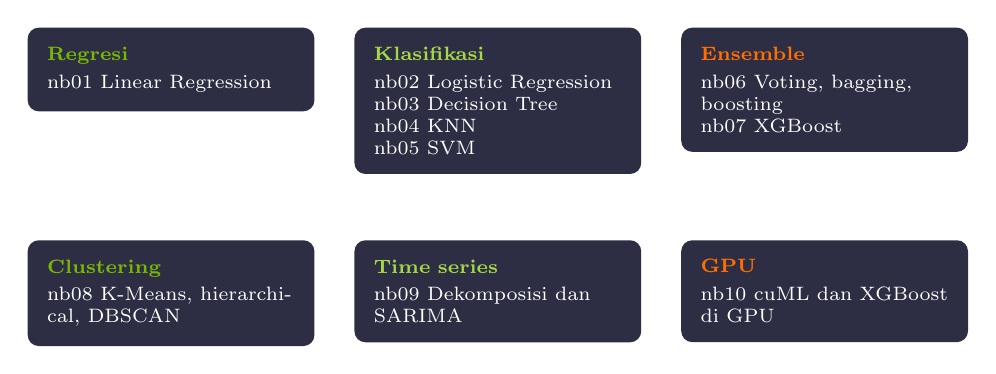
\begin{tikzpicture}[
    card/.style={fill=nvcard, rounded corners=4pt, inner sep=7pt, text width=3.15cm,
                 text=nvwhite, font=\scriptsize, anchor=north west, align=left}]
    \node[card] at (0,0)
      {{\bfseries\color{nvgreen}Regresi}\\[2pt] nb01 Linear Regression};
    \node[card] at (4.15,0)
      {{\bfseries\color{nvlightgreen}Klasifikasi}\\[2pt]
       nb02 Logistic Regression\\ nb03 Decision Tree\\ nb04 KNN\\ nb05 SVM};
    \node[card] at (8.3,0)
      {{\bfseries\color{nvorange}Ensemble}\\[2pt]
       nb06 Voting, bagging, boosting\\ nb07 XGBoost};
    \node[card] at (0,-2.7)
      {{\bfseries\color{nvgreen}Clustering}\\[2pt]
       nb08 K-Means, hierarchical, DBSCAN};
    \node[card] at (4.15,-2.7)
      {{\bfseries\color{nvlightgreen}Time series}\\[2pt]
       nb09 Dekomposisi dan SARIMA};
    \node[card] at (8.3,-2.7)
      {{\bfseries\color{nvorange}GPU}\\[2pt]
       nb10 cuML dan XGBoost di GPU};
  \end{tikzpicture}
  \end{center}
  \vspace{0.4em}
  {\footnotesize\color{nvgray}Sebelum notebook pertama kita bahas alur kerjanya dulu: bagaimana model
  belajar, dan bagaimana hasilnya diuji.}
\end{frame}

% ==========================================================
% ACT 1
% ==========================================================
\acttitle{Act 1}{Apa itu Machine Learning?}{Kalau aturannya tidak bisa ditulis, biarkan datanya yang bicara}

% ----------------------------------------------------------
% FRAME 4 — Intuisi: aturan tertulis vs belajar dari contoh
% ----------------------------------------------------------
\begin{frame}
  \intuisi{Aturan tertulis vs belajar dari contoh}
  \vspace{0.2em}
  \begin{columns}[T]
    \begin{column}{0.48\textwidth}
      \textbf{\color{nvred}Spam filter versi if/else}
      \vspace{0.4em}
      \begin{itemize}\setlength\itemsep{0.45em}
        \item Subjek memuat ``GRATIS'' $\rightarrow$ dikirim sebagai ``G R A T I S''
        \item Pengirim tidak dikenal $\rightarrow$ alamat baru dibuat tiap hari
        \item Lima tanda seru $\rightarrow$ dikurangi jadi dua
      \end{itemize}
    \end{column}
    \begin{column}{0.48\textwidth}
      \textbf{\color{nvgreen}Versi machine learning}
      \vspace{0.4em}
      \begin{itemize}\setlength\itemsep{0.45em}
        \item 10.000 email yang sudah ditandai spam atau bukan
        \item Model menyesuaikan parameternya untuk menangkap pola pada contoh itu
        \item Contoh baru masuk, polanya ikut diperbarui
      \end{itemize}
    \end{column}
  \end{columns}
  \vspace{0.4em}
  \nvbox{Intinya}{Machine learning adalah program yang aturannya dipelajari dari contoh,
  bukan ditulis tangan satu per satu.}
\end{frame}

% ----------------------------------------------------------
% FRAME 5 — Tiga jenis ML
% ----------------------------------------------------------
\begin{frame}{Tiga jenis machine learning}
  \begin{center}
    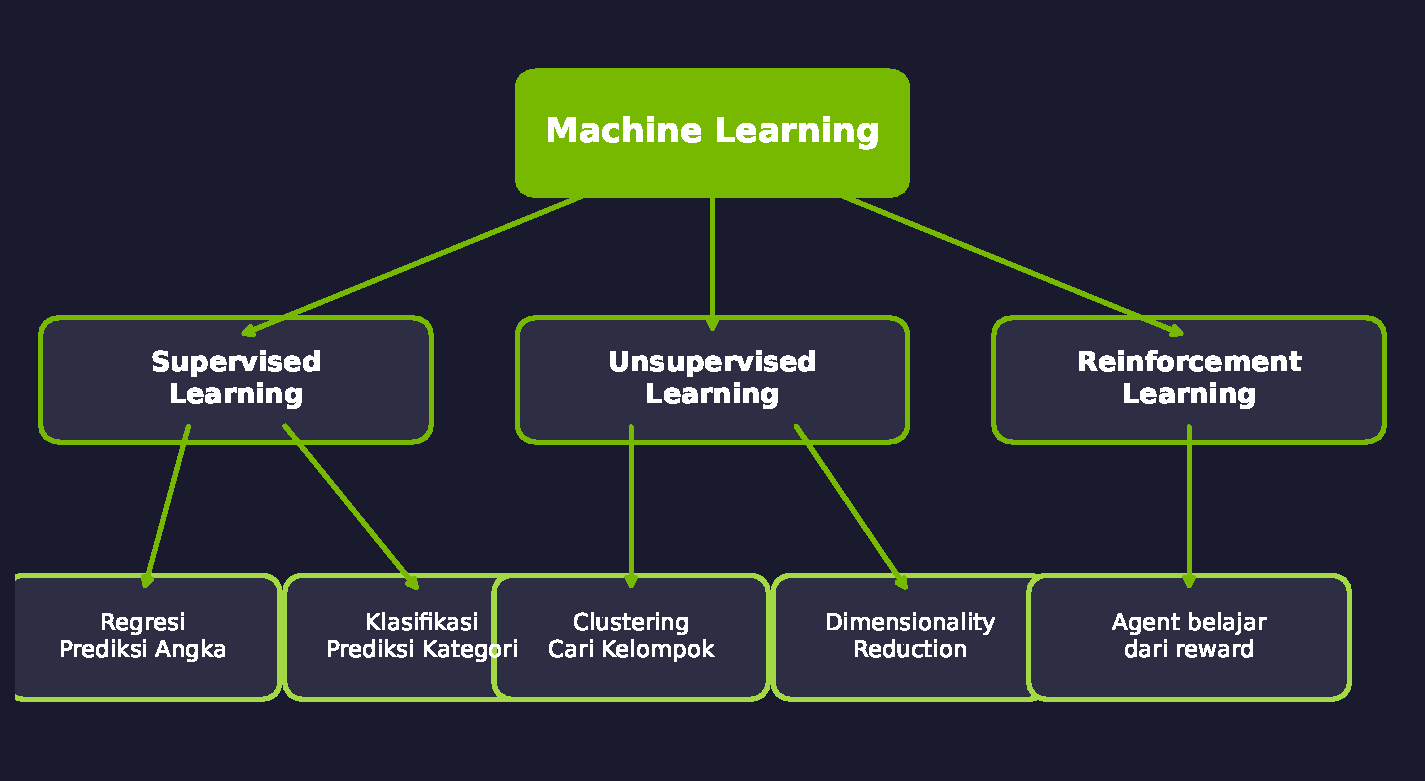
\includegraphics[width=0.62\textwidth, height=3.4cm, keepaspectratio]{figures/ml_types.pdf}
  \end{center}
  \begin{itemize}\setlength\itemsep{0.35em}
    \item \textbf{\color{nvgreen}Supervised}: setiap contoh punya jawabannya. Sembilan notebook
          pertama ada di sini.
    \item \textbf{\color{nvlightgreen}Unsupervised}: tanpa jawaban, model mencari struktur dalam
          data. Ini clustering di nb08.
    \item \textbf{\color{nvgray}Reinforcement}: belajar dari reward atas tindakannya. Hari ini
          hanya sebagai konteks.
  \end{itemize}
\end{frame}

% ----------------------------------------------------------
% FRAME 6 — Contoh sehari-hari
% ----------------------------------------------------------
\begin{frame}{Contoh yang kamu pakai tiap hari}
  \vspace{0.8em}
  \begin{center}
  {\small\renewcommand{\arraystretch}{1.25}
  \begin{tabular}{lll}
    \toprule
    \rowcolor{nvcard}\color{nvgreen}\textbf{Layanan} &
    \color{nvgreen}\textbf{Yang diprediksi} &
    \color{nvgreen}\textbf{Jenis tugas} \\
    \midrule
    Gmail & email ini spam atau bukan & klasifikasi \\
    \rowcolor{nvcard!60!nvbg} Google Maps & lama waktu tempuh & regresi \\
    Spotify & pendengar dengan selera mirip & clustering \\
    \rowcolor{nvcard!60!nvbg} Toko online & permintaan minggu depan & time series \\
    \bottomrule
  \end{tabular}}
  \end{center}
  \vspace{1.0em}
  {\footnotesize\color{nvgray}Keempat baris ini memakai kelompok model yang kita buka hari ini
  juga. Bedanya ada di ukuran data dan jumlah orang yang merawat sistemnya.}
\end{frame}

% ----------------------------------------------------------
% FRAME 7 — Tools
% ----------------------------------------------------------
\begin{frame}{Tools hari ini}
  \vspace{0.6em}
  \begin{columns}[T]
    \begin{column}{0.48\textwidth}
      \begin{itemize}\setlength\itemsep{0.55em}
        \item \textbf{\color{nvgreen}Python} --- bahasa yang dipakai sepanjang hari
        \item \textbf{\color{nvgreen}Google Colab (GPU T4)} --- menjalankan notebook tanpa
              instalasi di laptop
        \item \textbf{\color{nvgreen}pandas, matplotlib} --- memuat data, melihat isinya,
              membuat grafik
      \end{itemize}
    \end{column}
    \begin{column}{0.48\textwidth}
      \begin{itemize}\setlength\itemsep{0.55em}
        \item \textbf{\color{nvlightgreen}scikit-learn} --- hampir semua model klasik di modul
              ini
        \item \textbf{\color{nvlightgreen}XGBoost} --- boosting untuk data tabular (nb07)
        \item \textbf{\color{nvlightgreen}cuML} --- model klasik yang dijalankan di GPU (nb10)
      \end{itemize}
    \end{column}
  \end{columns}
  \vspace{1.0em}
  {\footnotesize\color{nvgray}Semua notebook memuat datanya langsung dari URL, jadi tidak ada
  file yang perlu kamu unggah dulu.}
\end{frame}

% ==========================================================
% ACT 2
% ==========================================================
\acttitle{Act 2}{\fontsize{24}{28}\selectfont\bfseries Bagaimana model belajar dan diuji?}{Dari kolom data mentah sampai satu angka yang layak dilaporkan}

% ----------------------------------------------------------
% FRAME 9 — Feature dan target
% ----------------------------------------------------------
\begin{frame}{Feature dan target}
  \vspace{0.2em}
  \begin{center}
  {\small\renewcommand{\arraystretch}{1.25}
  \begin{tabular}{rrr|r}
    \toprule
    \rowcolor{nvcard}\color{nvgreen}\texttt{TV} & \color{nvgreen}\texttt{radio} &
    \color{nvgreen}\texttt{newspaper} & \color{nvorange}\texttt{sales} \\
    \midrule
    230,1 & 37,8 & 69,2 & 22,1 \\
    \rowcolor{nvcard!60!nvbg} 44,5 & 39,3 & 45,1 & 10,4 \\
    17,2 & 45,9 & 69,3 & 9,3 \\
    \bottomrule
    \multicolumn{3}{c}{\color{nvgreen}\small tiga feature} &
    \multicolumn{1}{c}{\color{nvorange}\small target} \\
  \end{tabular}}
  \end{center}
  \vspace{0.3em}
  \begin{itemize}\setlength\itemsep{0.35em}
    \item \textbf{Feature} adalah kolom masukan yang dipakai model: belanja iklan di tiga kanal.
    \item \textbf{Target} adalah nilai yang mau diprediksi: penjualan.
    \item Targetnya berupa angka, jadi tugasnya regresi. Kalau targetnya kategori, itu
          klasifikasi dan targetnya disebut label kelas.
  \end{itemize}
\end{frame}

% ----------------------------------------------------------
% FRAME 10 — Intuisi: kenapa data dibagi
% ----------------------------------------------------------
\begin{frame}
  \intuisi{Kenapa data dibagi dua}
  \vspace{0.6em}
  \begin{columns}[T]
    \begin{column}{0.48\textwidth}
      \textbf{\color{nvlightgreen}Soal latihan}
      \vspace{0.4em}
      \begin{itemize}\setlength\itemsep{0.45em}
        \item Dikerjakan berulang sampai polanya kelihatan
        \item Jawabannya sudah ada di buku
      \end{itemize}
    \end{column}
    \begin{column}{0.48\textwidth}
      \textbf{\color{nvorange}Soal ujian}
      \vspace{0.4em}
      \begin{itemize}\setlength\itemsep{0.45em}
        \item Belum pernah dilihat sebelumnya
        \item Nilainya baru berarti kalau soalnya memang baru
      \end{itemize}
    \end{column}
  \end{columns}
  \vspace{0.8em}
  \nvbox{Intinya}{Data train dipakai untuk melatih model. Data test disimpan utuh dan dipakai
  sekali di akhir untuk menilai hasilnya.}
\end{frame}

% ----------------------------------------------------------
% FRAME 11 — Train / validation / test
% ----------------------------------------------------------
\begin{frame}{Data train, validation, dan test}
  \vspace{0.9em}
  \begin{center}
  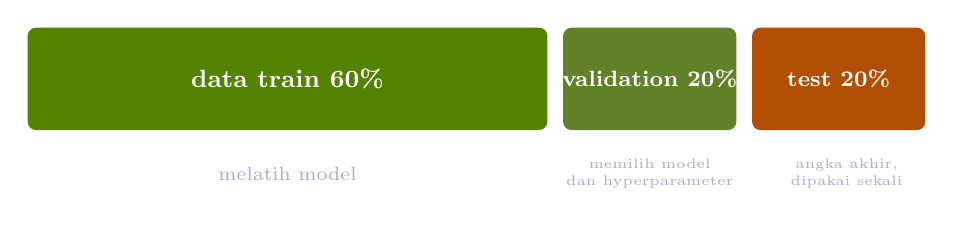
\begin{tikzpicture}[font=\small]
    \fill[nvgreen!70!black, rounded corners=3pt] (0,0) rectangle (6.6,1.3);
    \fill[nvlightgreen!60!black, rounded corners=3pt] (6.8,0) rectangle (9.0,1.3);
    \fill[nvorange!70!black, rounded corners=3pt] (9.2,0) rectangle (11.4,1.3);
    \node[text=nvwhite, font=\small\bfseries] at (3.3,0.65) {data train 60\%};
    \node[text=nvwhite, font=\footnotesize\bfseries] at (7.9,0.65) {validation 20\%};
    \node[text=nvwhite, font=\footnotesize\bfseries] at (10.3,0.65) {test 20\%};
    \node[text=nvgray, font=\scriptsize, align=center] at (3.3,-0.55) {melatih model};
    \node[text=nvgray, font=\tiny, align=center] at (7.9,-0.55)
      {memilih model\\ dan hyperparameter};
    \node[text=nvgray, font=\tiny, align=center] at (10.4,-0.55)
      {angka akhir,\\ dipakai sekali};
  \end{tikzpicture}
  \end{center}
  \vspace{1.0em}
  \begin{itemize}\setlength\itemsep{0.4em}
    \item Proporsinya bukan aturan baku; 60/20/20 dan 80/20 sama-sama umum.
    \item Kalau datanya sedikit, validation diganti cross-validation di data train.
  \end{itemize}
\end{frame}

% ----------------------------------------------------------
% FRAME 12 — Intuisi: leakage
% ----------------------------------------------------------
\begin{frame}
  \intuisi{Leakage: memakai informasi yang belum tersedia}
  \vspace{0.4em}
  \begin{columns}[T]
    \begin{column}{0.55\textwidth}
      \vspace{0.3em}
      \begin{itemize}\setlength\itemsep{0.55em}
        \item Tujuannya memprediksi respons nasabah sebelum telepon dilakukan.
        \item Kolom \texttt{duration} baru lengkap setelah panggilan berakhir.
        \item Memakai kolom itu membuat hasil evaluasi terlalu optimistis.
      \end{itemize}
      \vspace{0.5em}
      {\footnotesize\color{nvgray}Ini salah satu bentuk leakage. Bentuk lain kita bahas
      di nb02.}
    \end{column}
    \begin{column}{0.43\textwidth}
      \begin{center}
        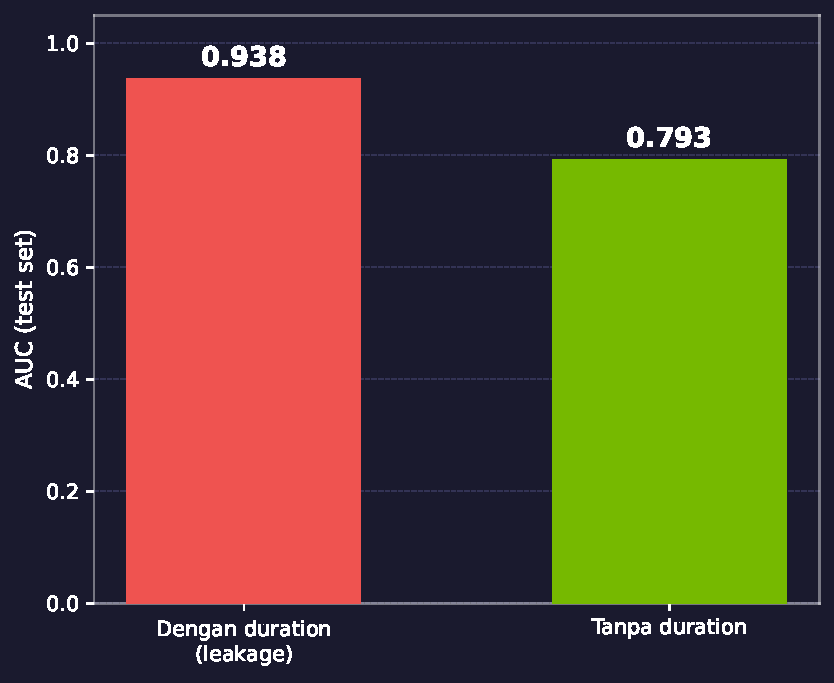
\includegraphics[width=\textwidth, height=4.3cm, keepaspectratio]{figures/leakage.pdf}
      \end{center}
    \end{column}
  \end{columns}
\end{frame}

% ----------------------------------------------------------
% FRAME 13 — Scaling
% ----------------------------------------------------------
\begin{frame}{Scaling: menyamakan rentang antar feature}
  \vspace{0.2em}
  \begin{center}
    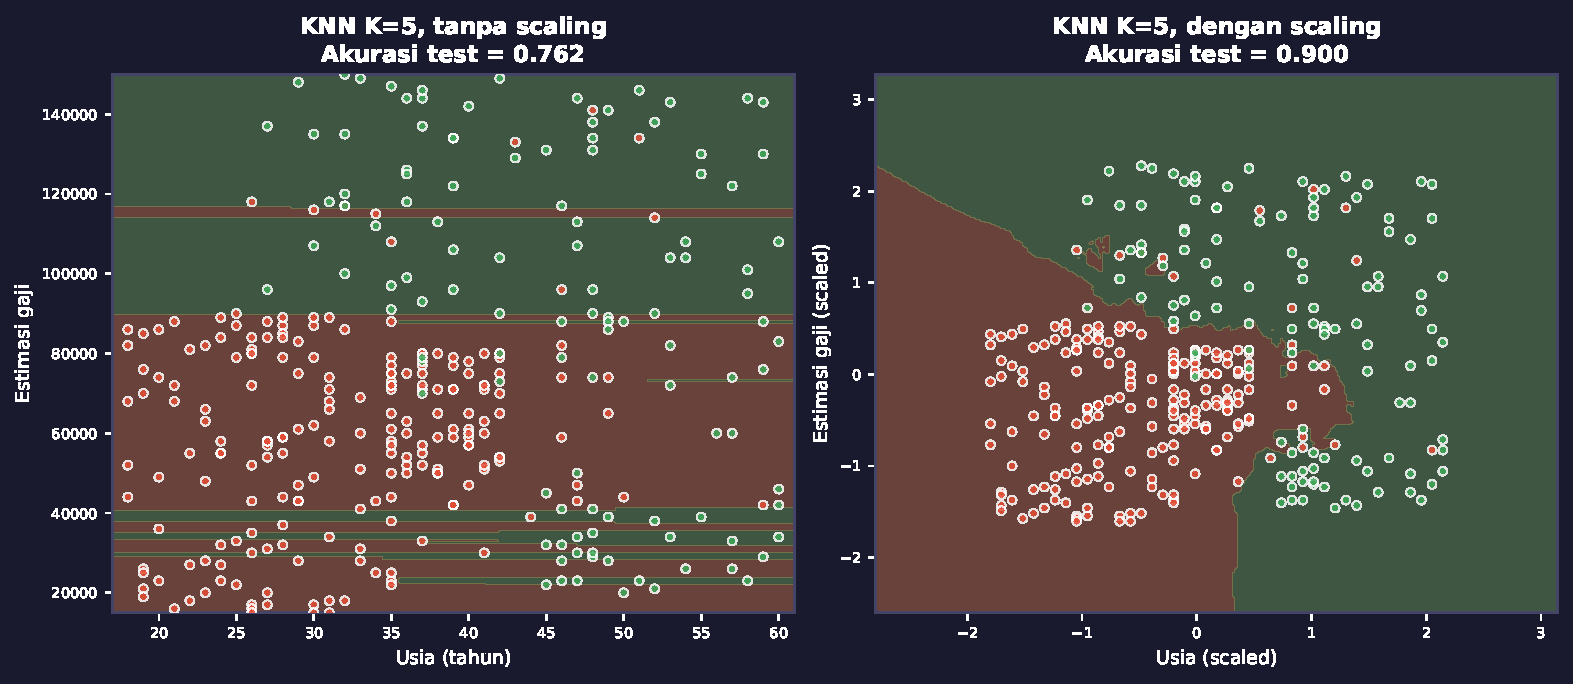
\includegraphics[width=0.88\textwidth, height=4.3cm, keepaspectratio]{figures/knn_scaling.pdf}
  \end{center}
  \vspace{0.2em}
  \begin{itemize}\setlength\itemsep{0.35em}
    \item Nilai gaji ada di puluhan ribu, umur di puluhan tahun. Tanpa scaling, selisih
          gaji mendominasi perhitungan jarak.
    \item Model berbasis jarak (KNN, SVM) dan model dengan penalti koefisien (logistic
          regression) butuh scaling; decision tree dan random forest tidak.
  \end{itemize}
\end{frame}

% ----------------------------------------------------------
% FRAME 14 — Intuisi: apa artinya belajar
% ----------------------------------------------------------
\begin{frame}
  \intuisi{Apa artinya ``belajar''}
  \vspace{0.4em}
  \begin{columns}[T]
    \begin{column}{0.52\textwidth}
      \begin{center}
      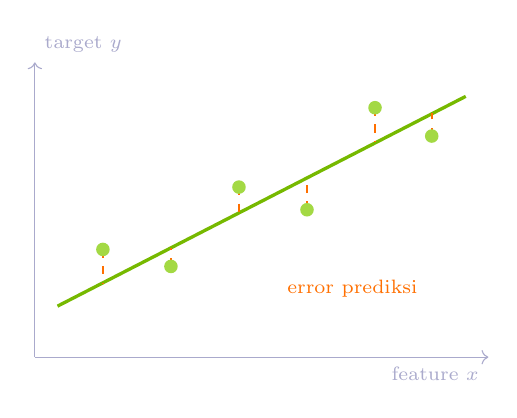
\begin{tikzpicture}[scale=0.72, font=\scriptsize]
        \draw[nvgray, ->] (0,0) -- (8,0) node[below left, text=nvgray] {feature $x$};
        \draw[nvgray, ->] (0,0) -- (0,5.2) node[above right, text=nvgray] {target $y$};
        \draw[nvgreen, line width=1.2pt] (0.4,0.9) -- (7.6,4.6);
        \foreach \x/\y/\yh in {1.2/1.9/1.31, 2.4/1.6/1.93, 3.6/3.0/2.55,
                               4.8/2.6/3.17, 6.0/4.4/3.79, 7.0/3.9/4.30} {
          \draw[nvorange, dashed, line width=0.7pt] (\x,\y) -- (\x,\yh);
          \fill[nvlightgreen] (\x,\y) circle (3.4pt);
        }
        \node[text=nvorange, font=\scriptsize] at (5.6,1.2) {error prediksi};
      \end{tikzpicture}
      \end{center}
    \end{column}
    \begin{column}{0.46\textwidth}
      \vspace{0.6em}
      \begin{itemize}\setlength\itemsep{0.5em}
        \item Garis hijau adalah prediksi model, titik hijau muda adalah data sebenarnya.
        \item Garis putus-putus oranye adalah error prediksi tiap baris.
        \item Melatih model berarti mengubah parameternya sampai total error itu sekecil
              mungkin.
      \end{itemize}
    \end{column}
  \end{columns}
\end{frame}

% ----------------------------------------------------------
% FRAME 15 — Loss regresi
% ----------------------------------------------------------
\begin{frame}{Loss: satu angka yang diminimalkan}
  \vspace{0.8em}
  \begin{center}
    \nvbox{Mean Squared Error}{
      \centerline{$\displaystyle \text{MSE} \;=\; \frac{1}{n}\sum_{i=1}^{n}\bigl(y_i - \hat{y}_i\bigr)^2$}
    }
  \end{center}
  \vspace{0.8em}
  \begin{itemize}\setlength\itemsep{0.45em}
    \item $y_i$ nilai sebenarnya, $\hat{y}_i$ prediksi model, $n$ jumlah baris.
    \item Selisihnya dikuadratkan, jadi error besar menyumbang jauh lebih banyak daripada
          beberapa error kecil.
    \item Pelatihan mencari parameter dengan MSE terkecil di data train. Angka yang
          dilaporkan tetap diambil dari data yang tidak dipakai melatih.
  \end{itemize}
\end{frame}

% ----------------------------------------------------------
% FRAME 16 — Underfitting dan overfitting
% ----------------------------------------------------------
\begin{frame}{Underfitting dan overfitting}
  \begin{center}
    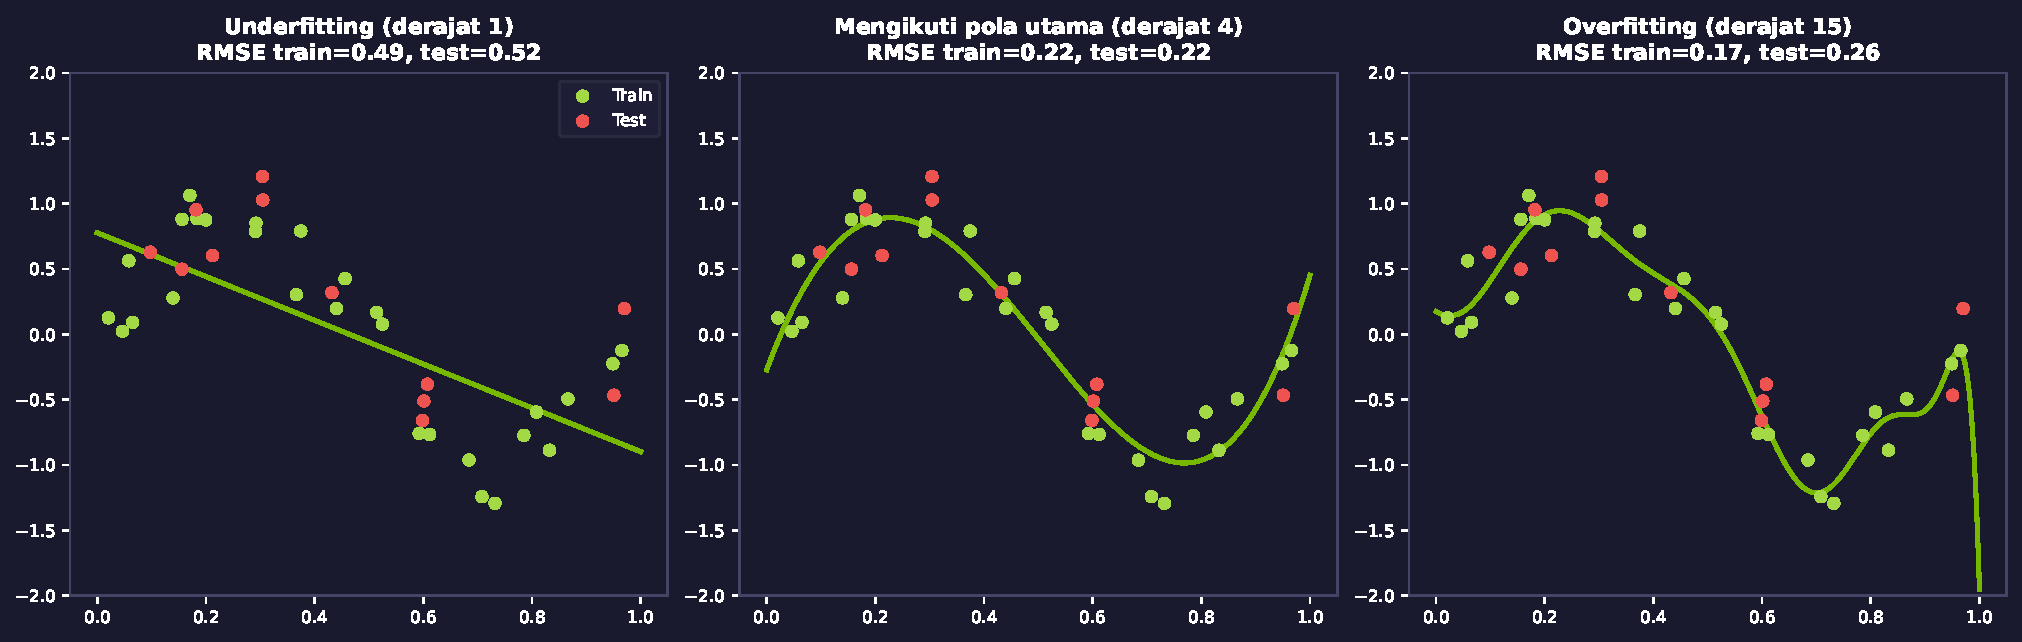
\includegraphics[width=\textwidth, height=3.8cm, keepaspectratio]{figures/bias_variance.pdf}
  \end{center}
  \begin{itemize}\setlength\itemsep{0.3em}
    \item \textbf{\color{nvorange}Kiri}: garis lurus terlalu sederhana untuk pola yang melengkung.
          Error di data train dan data test dua-duanya besar.
    \item \textbf{\color{nvgreen}Tengah}: masih mengikuti pola utama tanpa melewati semua titik.
    \item \textbf{\color{nvred}Kanan}: mengikuti hampir setiap titik, termasuk variasi acaknya.
          Error train turun, error test naik.
  \end{itemize}
\end{frame}

% ----------------------------------------------------------
% FRAME 17 — Bias-variance trade-off
% ----------------------------------------------------------
\begin{frame}{Bias--variance trade-off}
  \vspace{0.3em}
  \begin{columns}[T]
    \begin{column}{0.52\textwidth}
      \begin{center}
      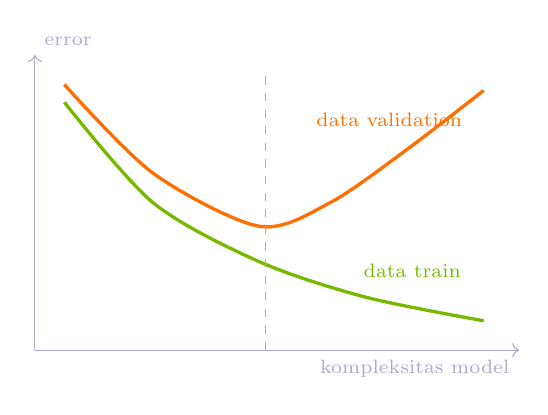
\begin{tikzpicture}[scale=0.75, font=\scriptsize]
        \draw[nvgray, ->] (0,0) -- (8.2,0) node[below left, text=nvgray] {kompleksitas model};
        \draw[nvgray, ->] (0,0) -- (0,5.0) node[above right, text=nvgray] {error};
        \draw[nvgreen, line width=1.2pt] plot[smooth]
          coordinates {(0.5,4.2)(2.0,2.5)(3.8,1.5)(5.6,0.9)(7.6,0.5)};
        \draw[nvorange, line width=1.2pt] plot[smooth]
          coordinates {(0.5,4.5)(2.0,3.0)(3.8,2.1)(5.0,2.5)(6.3,3.4)(7.6,4.4)};
        \draw[nvgray, dashed] (3.9,0) -- (3.9,4.7);
        \node[text=nvgreen, anchor=west] at (5.4,1.35) {data train};
        \node[text=nvorange, anchor=east] at (7.4,3.9) {data validation};
      \end{tikzpicture}
      \end{center}
    \end{column}
    \begin{column}{0.46\textwidth}
      \vspace{1.0em}
      \begin{itemize}\setlength\itemsep{0.6em}
        \item Model yang terlalu sederhana dapat melewatkan pola.
        \item Model yang terlalu peka terhadap data train dapat berubah banyak ketika sampel
              pelatihannya berubah.
        \item Error di data train hampir selalu turun saat model dibuat lebih rumit. Yang perlu
              dilihat adalah error di data yang tidak dipakai melatih.
      \end{itemize}
    \end{column}
  \end{columns}
\end{frame}

% ----------------------------------------------------------
% FRAME 18 — Cross-validation
% ----------------------------------------------------------
\begin{frame}{Cross-validation: menilai model lima kali}
  \begin{center}
  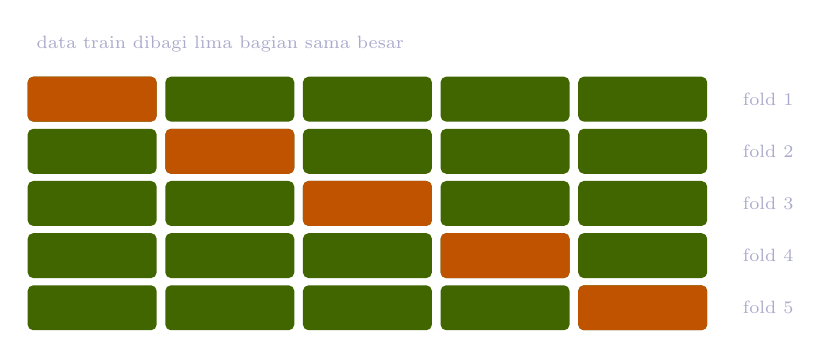
\begin{tikzpicture}[font=\scriptsize, scale=0.92, every node/.style={transform shape}]
    \foreach \r in {1,...,5} {
      \foreach \c in {0,...,4} {
        \fill[nvgreen!55!black, rounded corners=2pt]
          (\c*1.9, -\r*0.72) rectangle ++(1.78,0.62);
      }
      \node[text=nvgray, anchor=west] at (9.75, {-\r*0.72+0.31}) {fold \r};
    }
    \foreach \i in {1,...,5} {
      \fill[nvorange!75!black, rounded corners=2pt]
        ({(\i-1)*1.9}, -\i*0.72) rectangle ++(1.78,0.62);
    }
    \node[text=nvgray, anchor=west] at (0,0.35)
      {data train dibagi lima bagian sama besar};
  \end{tikzpicture}
  \end{center}
  \vspace{0.2em}
  \begin{itemize}\setlength\itemsep{0.3em}
    \item Tiap putaran, satu bagian (oranye) dipakai menilai, empat sisanya untuk melatih.
    \item Skornya rata-rata lima putaran, jadi tidak bergantung pada satu potongan data yang
          kebetulan mudah.
    \item Data test tetap di luar semua ini.
  \end{itemize}
\end{frame}

% ----------------------------------------------------------
% FRAME 19 — Baseline
% ----------------------------------------------------------
\begin{frame}{Baseline: pembanding paling sederhana}
  \vspace{0.5em}
  \begin{itemize}\setlength\itemsep{0.5em}
    \item \textbf{Regresi}: prediksi satu nilai konstan, yaitu rata-rata target di data train.
    \item \textbf{Klasifikasi}: prediksi kelas mayoritas untuk semua baris.
    \item Di \texttt{income\_evaluation.csv}, 76\% baris berlabel \texttt{<=50K}. Model yang
          memprediksi kelas itu untuk semua baris sudah dapat akurasi 76\%.
  \end{itemize}
  \vspace{0.9em}
  \jebakan{akurasi 76\% pada data seperti itu belum menunjukkan apa pun. Hitung baseline
  lebih dulu, lalu lihat selisih hasil modelmu terhadap baseline.}
\end{frame}

% ----------------------------------------------------------
% FRAME 20 — Metrik regresi
% ----------------------------------------------------------
\begin{frame}{Metrik regresi: MAE, RMSE, R\texorpdfstring{$^2$}{2}}
  \vspace{0.5em}
  \begin{center}
  {\small\renewcommand{\arraystretch}{1.25}
  \begin{tabular}{p{1.5cm} p{9.2cm}}
    \toprule
    \rowcolor{nvcard}\color{nvgreen}\textbf{Metrik} & \color{nvgreen}\textbf{Arti} \\
    \midrule
    MAE & rata-rata selisih absolut prediksi dan nilai sebenarnya; satuannya sama dengan
          target \\
    \rowcolor{nvcard!60!nvbg} RMSE & akar dari rata-rata kuadrat error; lebih peka terhadap error
          besar daripada MAE karena perhitungannya memakai kuadrat error \\
    $R^2$ & membandingkan error kuadrat model dengan prediksi konstan berupa rata-rata target;
          1 berarti prediksi tepat, 0 setara pembanding itu, negatif berarti lebih buruk \\
    \bottomrule
  \end{tabular}}
  \end{center}
  \vspace{0.7em}
  {\footnotesize\color{nvgray}Pilih metrik sebelum melatih model, bukan setelah melihat hasilnya.}
\end{frame}

% ----------------------------------------------------------
% FRAME 21 — Confusion matrix
% ----------------------------------------------------------
\begin{frame}{Confusion matrix: dua jenis kesalahan}
  \vspace{0.2em}
  {\footnotesize\color{nvgray}Positif berarti kondisi yang ingin dideteksi, bukan hasil yang baik.}
  \vspace{0.4em}
  \begin{center}
  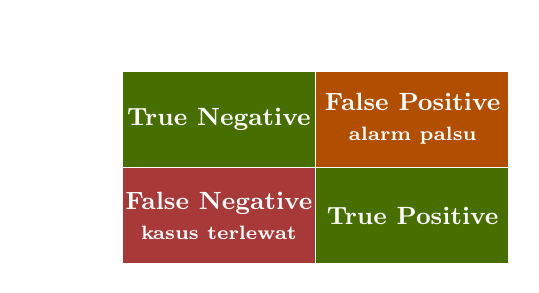
\begin{tikzpicture}[scale=0.82, font=\small]
    \node[text=nvwhite, font=\footnotesize\bfseries] at (1.5,3.4) {Prediksi: Tidak};
    \node[text=nvwhite, font=\footnotesize\bfseries] at (4.5,3.4) {Prediksi: Ya};
    \node[text=nvwhite, font=\footnotesize\bfseries, rotate=90] at (-1.2,1.5) {Asli};
    \node[text=nvwhite, font=\footnotesize, anchor=east] at (-0.2,2.25) {Tidak};
    \node[text=nvwhite, font=\footnotesize, anchor=east] at (-0.2,0.75) {Ya};
    \fill[nvgreen!60!black] (0,1.5) rectangle (3,3);
    \node[text=nvwhite, font=\small\bfseries] at (1.5,2.25) {True Negative};
    \fill[nvorange!70!black] (3,1.5) rectangle (6,3);
    \node[text=nvwhite, font=\small\bfseries, align=center] at (4.5,2.25)
      {False Positive\\ \scriptsize alarm palsu};
    \fill[nvred!70!black] (0,0) rectangle (3,1.5);
    \node[text=nvwhite, font=\small\bfseries, align=center] at (1.5,0.75)
      {False Negative\\ \scriptsize kasus terlewat};
    \fill[nvgreen!60!black] (3,0) rectangle (6,1.5);
    \node[text=nvwhite, font=\small\bfseries] at (4.5,0.75) {True Positive};
    \draw[nvwhite, thick] (0,0) rectangle (6,3);
    \draw[nvwhite] (3,0) -- (3,3);
    \draw[nvwhite] (0,1.5) -- (6,1.5);
  \end{tikzpicture}
  \end{center}
  \vspace{0.4em}
  {\footnotesize\color{nvgray}Akurasi menjumlahkan dua kotak hijau saja. Dua kotak sisanya punya
  biaya yang berbeda, dan itu yang menentukan metrik mana yang kita pakai.}
\end{frame}

% ----------------------------------------------------------
% FRAME 22 — Precision, recall, F1, ROC-AUC
% ----------------------------------------------------------
\begin{frame}{Precision, recall, F1, dan ROC-AUC}
  \vspace{0.2em}
  \begin{columns}[T]
    \begin{column}{0.5\textwidth}
      \begin{itemize}\setlength\itemsep{0.3em}
        \item \textbf{\color{nvgreen}Precision}: dari yang diprediksi positif, berapa bagian yang
              benar positif.
        \item \textbf{\color{nvlightgreen}Recall}: dari yang benar-benar positif, berapa bagian
              yang tertangkap.
        \item \textbf{F1}: rata-rata harmonik precision dan recall, turun tajam kalau salah satu
              rendah.
        \item \textbf{ROC-AUC}: peluang model memberi skor lebih tinggi pada satu contoh positif
              dibanding satu contoh negatif.
      \end{itemize}
    \end{column}
    \begin{column}{0.48\textwidth}
      \begin{center}
        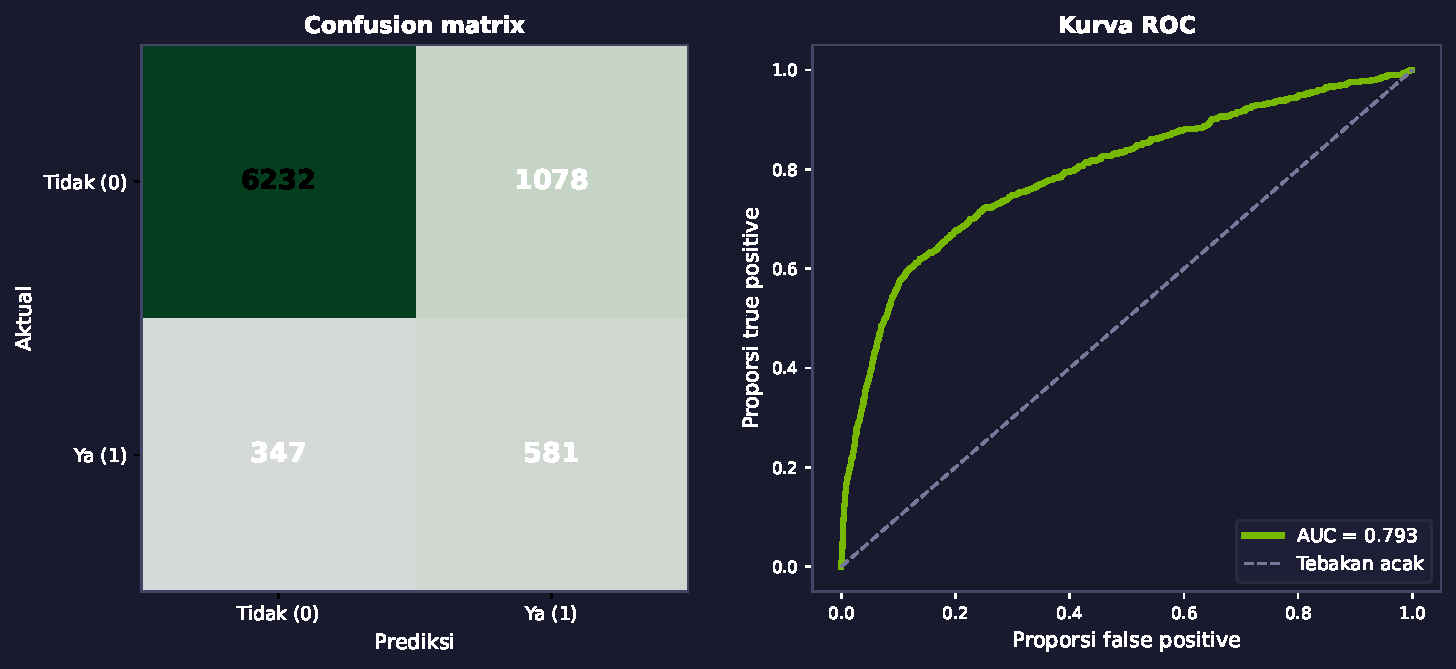
\includegraphics[width=\textwidth, height=3.9cm, keepaspectratio]{figures/metrics_roc.pdf}
      \end{center}
      {\scriptsize\color{nvgray}Model logistic regression pada data banking tanpa
      \texttt{duration}.}
    \end{column}
  \end{columns}
\end{frame}

% ----------------------------------------------------------
% FRAME 23 — Ringkasan alur kerja
% ----------------------------------------------------------
\begin{frame}{Alur kerja yang dipakai di sepuluh notebook}
  \vspace{0.5em}
  \begin{enumerate}\setlength\itemsep{0.42em}
    \item Definisikan masalahnya dan metrik yang akan dilaporkan.
    \item Siapkan data: periksa nilai kosong, outlier (pencilan), dan kolom yang tidak tersedia
          saat prediksi.
    \item Split data train, validation, dan test.
    \item Latih model di data train.
    \item Bandingkan hasilnya dengan baseline.
    \item Tuning hyperparameter dengan cross-validation di data train.
    \item Uji sekali di data test, lalu laporkan angka itu.
  \end{enumerate}
  \vspace{0.6em}
  {\footnotesize\color{nvgray}Langkah 2 dan 3 memakan waktu paling banyak. Langkah 7 yang paling
  sering dilewati.}
\end{frame}

% ==========================================================
% ACT 3
% ==========================================================
\acttitle{Act 3}{\fontsize{24}{28}\selectfont\bfseries Bagaimana memprediksi nilai?}{Dari satu garis lurus sampai deret waktu dengan pola musiman}

% ----------------------------------------------------------
% FRAME 25 — Intuisi: linear regression
% ----------------------------------------------------------
\begin{frame}
  \intuisi{Suhu naik, es krim terjual lebih banyak}
  \vspace{0.3em}
  \begin{columns}[T]
    \begin{column}{0.52\textwidth}
      \begin{center}
        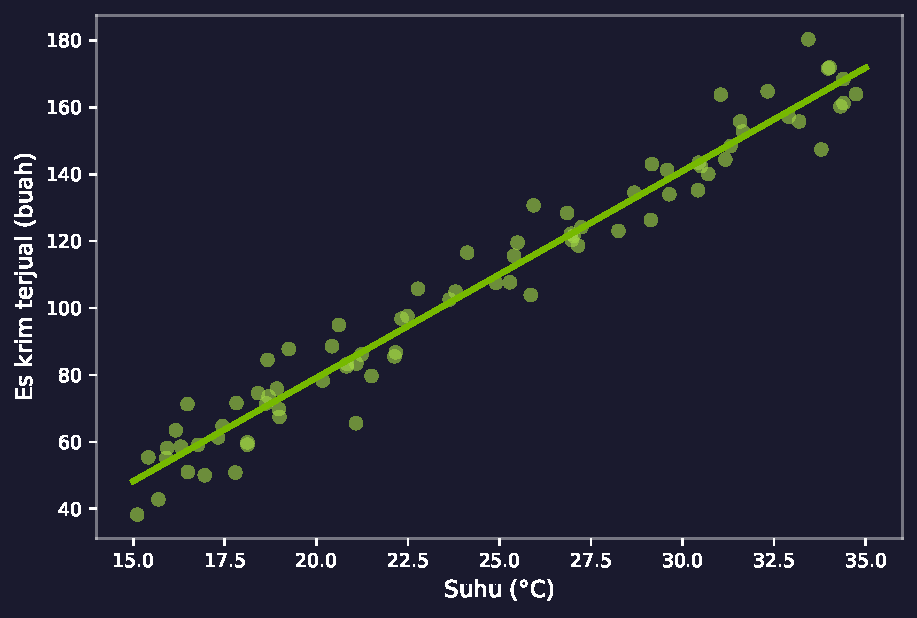
\includegraphics[width=\textwidth, height=4.2cm, keepaspectratio]{figures/regression_line.pdf}
      \end{center}
    \end{column}
    \begin{column}{0.46\textwidth}
      \vspace{0.2em}
      \begin{itemize}\setlength\itemsep{0.45em}
        \item Titik hijau adalah catatan harian: suhu hari itu dan jumlah es krim terjual.
        \item Banyak garis bisa ditarik di antara titik-titik itu. Yang dipilih hanya satu.
      \end{itemize}
      \vspace{0.6em}
      \nvbox{Intinya}{Linear regression mencari garis yang total error prediksinya paling kecil.}
    \end{column}
  \end{columns}
\end{frame}

% ----------------------------------------------------------
% FRAME 26 — Mekanisme linear regression
% ----------------------------------------------------------
\begin{frame}{Linear regression: satu garis, dua parameter}
  \vspace{0.5em}
  \begin{center}
    \nvbox{Bentuk modelnya}{
      \centerline{$\displaystyle \hat{y} \;=\; w\,x + b$}
    }
  \end{center}
  \vspace{0.7em}
  \begin{itemize}\setlength\itemsep{0.45em}
    \item $w$ adalah kemiringan (slope): berapa banyak prediksi berubah tiap satu satuan
          kenaikan $x$.
    \item $b$ adalah intercept: nilai prediksi saat $x = 0$.
    \item Dengan banyak feature, tiap feature punya satu $w$ sendiri:
          $\hat{y} = w_1 x_1 + w_2 x_2 + \dots + w_k x_k + b$.
    \item Pelatihan memilih $w$ dan $b$ yang membuat MSE di data train terkecil.
  \end{itemize}
\end{frame}

% ----------------------------------------------------------
% FRAME 27 — Kapan pakai & jebakan linear regression
% ----------------------------------------------------------
\begin{frame}{Linear regression: kapan pakai dan jebakannya}
  \vspace{0.4em}
  \kapan{
    \item hubungan feature dan target mendekati lurus
    \item kamu perlu model yang koefisiennya bisa dibaca dan dijelaskan
    \item jumlah feature masih sedikit
  }{
    \item polanya jelas melengkung atau berjenjang
    \item ada outlier (pencilan) yang menarik garisnya
    \item pengaruh satu feature bergantung pada feature lain
  }
  \vspace{1.0em}
  \jebakan{koefisien besar tidak berarti feature itu penyebabnya. Selain itu $x = 0$ sering
  berada di luar rentang data, jadi intercept belum tentu punya arti nyata.}
\end{frame}

% ----------------------------------------------------------
% FRAME 28 — Regularisasi
% ----------------------------------------------------------
\begin{frame}{Regularisasi: membatasi ukuran koefisien}
  \vspace{0.4em}
  {\small Regularisasi (regularization) membatasi kompleksitas model agar tidak terlalu
  menyesuaikan diri dengan data train.}
  \vspace{0.5em}
  \begin{center}
    \nvbox{Yang diminimalkan}{
      \centerline{loss di data train \;$+$\; penalti atas ukuran koefisien}
    }
  \end{center}
  \vspace{0.5em}
  \begin{itemize}\setlength\itemsep{0.4em}
    \item \textbf{\color{nvgreen}Ridge} mengecilkan semua koefisien, jarang sampai nol.
    \item \textbf{\color{nvlightgreen}Lasso} bisa menolkan koefisien yang tidak berguna,
          jadi sekaligus menyeleksi feature.
    \item Kekuatan penaltinya dipilih dengan cross-validation. Penalti yang terlalu kuat
          membuat model melewatkan pola penting.
  \end{itemize}
\end{frame}

% ----------------------------------------------------------
% FRAME 29 — Intuisi: time series
% ----------------------------------------------------------
\begin{frame}
  \intuisi{Time series: urutan waktunya ikut menentukan}
  \vspace{0.2em}
  \begin{columns}[T]
    \begin{column}{0.47\textwidth}
      \vspace{0.3em}
      \begin{itemize}\setlength\itemsep{0.4em}
        \item \textbf{\color{nvorange}Trend}: arah jangka panjang, di sini naik terus.
        \item \textbf{\color{nvgreen}Pola musiman}: naik-turun yang berulang tiap 12 bulan.
        \item \textbf{\color{nvgray}Noise}: sisa gerakan yang tidak dijelaskan keduanya.
      \end{itemize}
      \vspace{0.5em}
      \nvbox{Intinya}{Urutan waktu adalah bagian dari datanya, jadi barisnya tidak boleh
      diacak seperti data tabular biasa.}
    \end{column}
    \begin{column}{0.51\textwidth}
      \begin{center}
        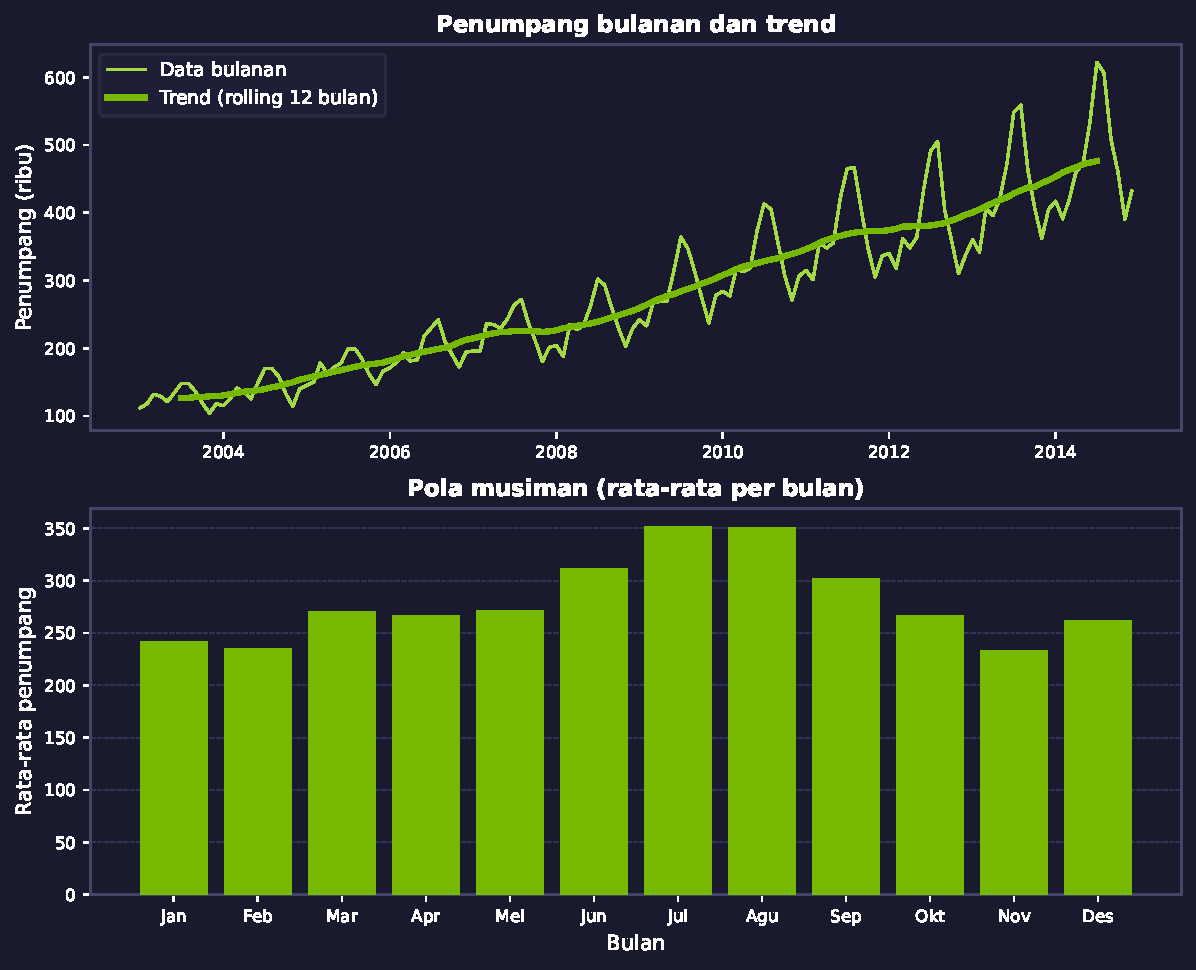
\includegraphics[width=\textwidth, height=5.2cm, keepaspectratio]{figures/timeseries.pdf}
      \end{center}
    \end{column}
  \end{columns}
\end{frame}

% ----------------------------------------------------------
% FRAME 30 — Stasioner dan differencing
% ----------------------------------------------------------
\begin{frame}{Stasioner dan differencing}
  \vspace{0.2em}
  \begin{center}
  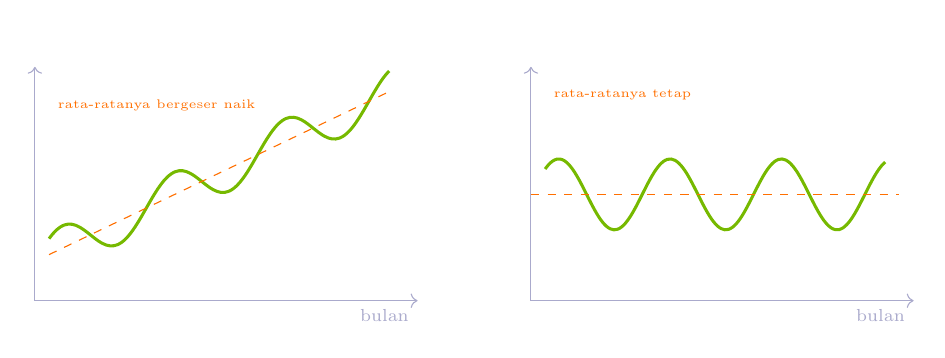
\begin{tikzpicture}[font=\scriptsize, scale=0.9, every node/.style={transform shape}]
    % kiri: deret asli
    \draw[nvgray, ->] (0,0) -- (5.4,0) node[below left, text=nvgray] {bulan};
    \draw[nvgray, ->] (0,0) -- (0,3.3);
    \draw[nvgreen, line width=1.1pt, domain=0.2:5.0, samples=90, smooth]
      plot (\x, {0.48*\x + 0.32*sin(4*\x r) + 0.55});
    \draw[nvorange, dashed] (0.2,0.65) -- (5.0,2.95);
    \node[text=nvwhite, font=\scriptsize] at (2.6,3.65) {deret asli};
    \node[text=nvorange, font=\tiny, anchor=west] at (0.2,2.75) {rata-ratanya bergeser naik};
    % kanan: setelah differencing
    \draw[nvgray, ->] (7.0,0) -- (12.4,0) node[below left, text=nvgray] {bulan};
    \draw[nvgray, ->] (7.0,0) -- (7.0,3.3);
    \draw[nvgreen, line width=1.1pt, domain=7.2:12.0, samples=90, smooth]
      plot (\x, {1.5 + 0.5*sin(4*(\x-7.0) r)});
    \draw[nvorange, dashed] (7.0,1.5) -- (12.2,1.5)
      node[anchor=west, text=nvorange, font=\tiny] {};
    \node[text=nvwhite, font=\scriptsize] at (9.7,3.65) {selisih antar bulan};
    \node[text=nvorange, font=\tiny, anchor=west] at (7.2,2.9) {rata-ratanya tetap};
  \end{tikzpicture}
  \end{center}
  \vspace{0.7em}
  \begin{itemize}\setlength\itemsep{0.35em}
    \item Deret disebut \textbf{stasioner} kalau sifat statistiknya tetap terhadap pergeseran
          waktu. Grafik yang tampak datar belum membuktikannya.
    \item \textbf{Differencing} memakai selisih antar bulan sebagai deret baru, supaya
          rata-ratanya tidak lagi bergeser.
  \end{itemize}
\end{frame}

% ----------------------------------------------------------
% FRAME 31 — SARIMA dan interval prediksi
% ----------------------------------------------------------
\begin{frame}{SARIMA dan interval prediksi}
  \vspace{0.1em}
  {\footnotesize\color{nvlightgreen}Seasonal AutoRegressive Integrated Moving Average}
  \vspace{0.3em}
  \begin{columns}[T]
    \begin{column}{0.38\textwidth}
      \begin{itemize}\setlength\itemsep{0.35em}
        \item \textbf{AR}: pakai nilai bulan-bulan sebelumnya.
        \item \textbf{I}: differencing seperti slide tadi.
        \item \textbf{MA}: pakai error prediksi sebelumnya.
        \item \textbf{S}: ulangi ketiganya pada jarak 12 bulan.
      \end{itemize}
    \end{column}
    \begin{column}{0.60\textwidth}
      \begin{center}
      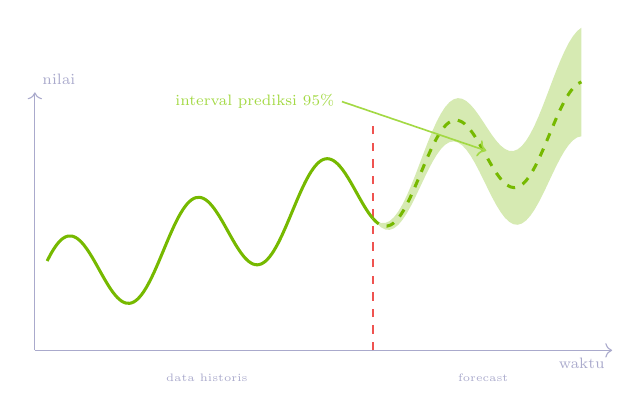
\begin{tikzpicture}[font=\scriptsize, scale=0.78, every node/.style={transform shape}]
        \draw[nvgray, ->] (0,0) -- (9.4,0) node[below left, text=nvgray] {waktu};
        \draw[nvgray, ->] (0,0) -- (0,4.2) node[above right, text=nvgray] {nilai};
        \draw[nvred, dashed, line width=0.8pt] (5.5,0) -- (5.5,3.7);
        \node[text=nvgray, font=\tiny] at (2.8,-0.45) {data historis};
        \node[text=nvgray, font=\tiny] at (7.3,-0.45) {forecast};
        \fill[nvgreen, opacity=0.30]
          plot[domain=5.5:8.9, samples=50]
            (\x, {0.3*\x + 0.7*sin(3.0*\x r) + 1.0 + 0.26*(\x-5.5)})
          -- plot[domain=8.9:5.5, samples=50]
            (\x, {0.3*\x + 0.7*sin(3.0*\x r) + 1.0 - 0.26*(\x-5.5)})
          -- cycle;
        \draw[nvgreen, line width=1.1pt, domain=0.2:5.5, samples=80, smooth]
          plot (\x, {0.3*\x + 0.7*sin(3.0*\x r) + 1.0});
        \draw[nvgreen, dashed, line width=1.1pt, domain=5.5:8.9, samples=60, smooth]
          plot (\x, {0.3*\x + 0.7*sin(3.0*\x r) + 1.0});
        \node[text=nvlightgreen, font=\scriptsize, anchor=east] (ip) at (5.0,4.05)
          {interval prediksi 95\%};
        \draw[nvlightgreen, ->, line width=0.6pt] (ip.east) -- (7.35,3.25);
      \end{tikzpicture}
      \end{center}
    \end{column}
  \end{columns}
  \vspace{0.2em}
  {\footnotesize\color{nvgray}Pita hijau adalah interval prediksi: rentang untuk nilai bulan
  berikutnya. Cakupan 95\% berlaku sejauh asumsi modelnya cocok dengan datanya.}
\end{frame}

% ----------------------------------------------------------
% FRAME 32 — Evaluasi time series
% ----------------------------------------------------------
\begin{frame}{Evaluasi time series: split kronologis}
  \vspace{0.7em}
  \begin{center}
  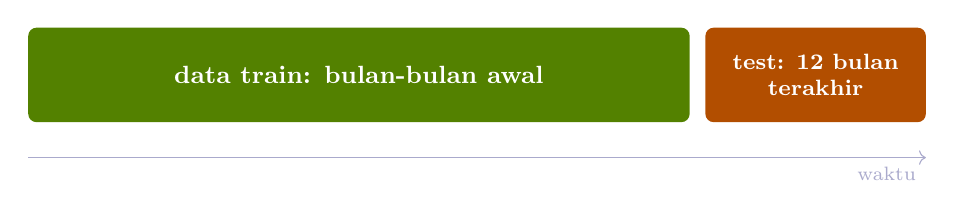
\begin{tikzpicture}[font=\small]
    \fill[nvgreen!70!black, rounded corners=3pt] (0,0) rectangle (8.4,1.2);
    \fill[nvorange!70!black, rounded corners=3pt] (8.6,0) rectangle (11.4,1.2);
    \node[text=nvwhite, font=\small\bfseries] at (4.2,0.6) {data train: bulan-bulan awal};
    \node[text=nvwhite, font=\footnotesize\bfseries, align=center] at (10.0,0.6)
      {test: 12 bulan\\ terakhir};
    \draw[nvgray, ->] (0,-0.45) -- (11.4,-0.45)
      node[below left, text=nvgray, font=\scriptsize] {waktu};
  \end{tikzpicture}
  \end{center}
  \vspace{0.9em}
  \begin{itemize}\setlength\itemsep{0.35em}
    \item Potongannya mengikuti waktu, bukan diacak. Model tidak boleh melihat bulan yang
          lebih baru daripada bulan yang diprediksi.
    \item \textbf{Baseline seasonal naive}: prediksi bulan ini sama dengan nilai bulan yang
          sama tahun lalu. SARIMA baru menarik kalau mengalahkan ini.
    \item \textbf{MAPE} adalah rata-rata error relatif dalam persen. Angkanya menyesatkan
          kalau nilai sebenarnya dekat nol.
  \end{itemize}
\end{frame}

% ----------------------------------------------------------
% FRAME 33 — Ringkasan Act 3
% ----------------------------------------------------------
\begin{frame}{Ringkasan Act 3}
  \vspace{0.5em}
  \begin{itemize}\setlength\itemsep{0.5em}
    \item Regresi memprediksi nilai berupa angka. Linear regression mencari $w$ dan $b$ yang
          membuat total error prediksi terkecil.
    \item Koefisien memberi arah dan besar pengaruh menurut model, bukan bukti sebab-akibat.
    \item Regularisasi menambah penalti atas ukuran koefisien; Lasso bisa menolkan koefisien
          yang tidak berguna.
    \item Pada time series, urutan waktu ikut menentukan: split kronologis, differencing untuk
          menstabilkan rata-rata, dan seasonal naive sebagai baseline.
  \end{itemize}
  \vspace{0.7em}
  {\footnotesize\color{nvgray}nb01 memakai Advertising, nb09 memakai SeaPlaneTravel.}
\end{frame}

% ==========================================================
% ACT 4
% ==========================================================
\acttitle{Act 4}{\fontsize{24}{28}\selectfont\bfseries Bagaimana memprediksi kategori?}{Empat model, empat cara menarik batas keputusan}

% ----------------------------------------------------------
% FRAME 35 — Regresi dan klasifikasi
% ----------------------------------------------------------
\begin{frame}{Regresi dan klasifikasi}
  \vspace{0.1em}
  \begin{columns}[T]
    \begin{column}{0.48\textwidth}
      \centering
      \textbf{\color{nvorange}Regresi}\\[0.3em]
      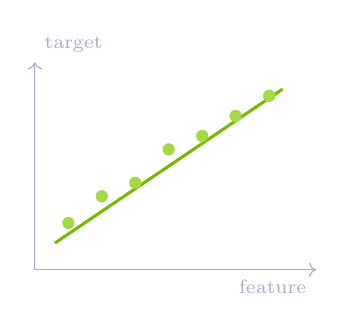
\begin{tikzpicture}[scale=0.85, font=\scriptsize]
        \draw[nvgray, ->] (0,0) -- (4.2,0) node[below left, text=nvgray] {feature};
        \draw[nvgray, ->] (0,0) -- (0,3.1) node[above right, text=nvgray] {target};
        \draw[nvgreen, line width=1.1pt] (0.3,0.4) -- (3.7,2.7);
        \foreach \x/\y in {0.5/0.7, 1.0/1.1, 1.5/1.3, 2.0/1.8, 2.5/2.0, 3.0/2.3, 3.5/2.6}
          \fill[nvlightgreen] (\x,\y) circle (2.6pt);
      \end{tikzpicture}\\[0.4em]
      {\small Keluarannya satu angka}\\[0.2em]
      {\footnotesize\color{nvgray}lama waktu tempuh, penjualan}
    \end{column}
    \begin{column}{0.48\textwidth}
      \centering
      \textbf{\color{nvgreen}Klasifikasi}\\[0.3em]
      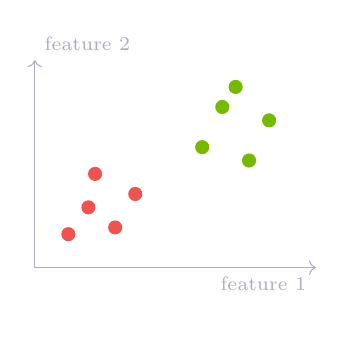
\begin{tikzpicture}[scale=0.85, font=\scriptsize]
        \draw[nvgray, ->] (0,0) -- (4.2,0) node[below left, text=nvgray] {feature 1};
        \draw[nvgray, ->] (0,0) -- (0,3.1) node[above right, text=nvgray] {feature 2};
        \foreach \x/\y in {0.5/0.5, 0.8/0.9, 1.2/0.6, 1.5/1.1, 0.9/1.4}
          \fill[nvred] (\x,\y) circle (3pt);
        \foreach \x/\y in {2.5/1.8, 2.8/2.4, 3.2/1.6, 3.5/2.2, 3.0/2.7}
          \fill[nvgreen] (\x,\y) circle (3pt);
        \draw[nvwhite, dashed] (2.05,0.1) -- (2.05,2.9);
        \node[text=nvwhite, font=\tiny, anchor=north] at (2.05,-0.55) {batas keputusan};
      \end{tikzpicture}\\[0.4em]
      {\small Keluarannya label kelas}\\[0.2em]
      {\footnotesize\color{nvgray}spam atau bukan, respons ya atau tidak}
    \end{column}
  \end{columns}
  \vspace{0.1em}
  {\footnotesize\color{nvgray}Alur kerjanya sama seperti Act 2. Yang berubah adalah bentuk
  keluaran model dan metrik yang dipakai menilainya.}
\end{frame}

% ----------------------------------------------------------
% FRAME 36 — Intuisi: logistic regression
% ----------------------------------------------------------
\begin{frame}
  \intuisi{Logistic regression: skor jadi probabilitas}
  \vspace{0.2em}
  \begin{center}
  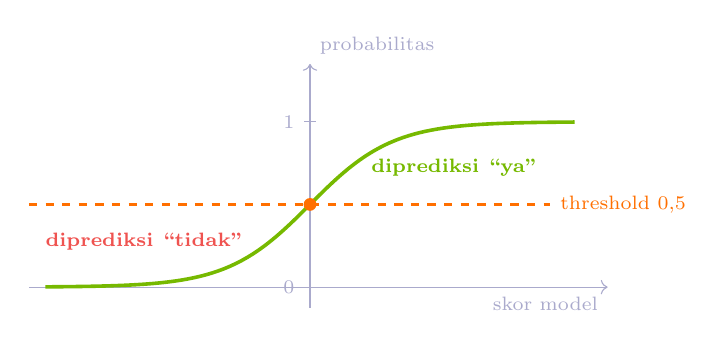
\begin{tikzpicture}[scale=1.05, font=\scriptsize]
    \draw[nvgray, ->] (-3.4,0) -- (3.6,0) node[below left, text=nvgray] {skor model};
    \draw[nvgray, ->] (0,-0.25) -- (0,2.7) node[above right, text=nvgray] {probabilitas};
    \draw[nvgray] (-0.07,0) node[left, text=nvgray] {0} -- (0.07,0);
    \draw[nvgray] (-0.07,2) node[left, text=nvgray] {1} -- (0.07,2);
    \draw[nvgreen, line width=1.3pt, domain=-3.2:3.2, samples=90]
      plot (\x, {2/(1+exp(-2*\x))});
    \draw[nvorange, dashed, line width=0.9pt] (-3.4,1) -- (2.9,1)
      node[right, text=nvorange, font=\scriptsize] {threshold 0,5};
    \fill[nvorange] (0,1) circle (2.2pt);
    \node[text=nvred, font=\scriptsize\bfseries] at (-2.0,0.55) {diprediksi ``tidak''};
    \node[text=nvgreen, font=\scriptsize\bfseries] at (1.75,1.45) {diprediksi ``ya''};
  \end{tikzpicture}
  \end{center}
  \vspace{0.3em}
  \nvbox{Intinya}{Model menghitung satu skor dari semua feature, lalu fungsi sigmoid memampatkan
  skor itu menjadi angka antara 0 dan 1 yang dibaca sebagai probabilitas kelas positif.}
\end{frame}

% ----------------------------------------------------------
% FRAME 37 — Mekanisme logistic regression
% ----------------------------------------------------------
\begin{frame}{Logistic regression: threshold dan data timpang}
  \vspace{0.5em}
  \begin{itemize}\setlength\itemsep{0.45em}
    \item Keluaran modelnya probabilitas. Label kelas muncul setelah probabilitas itu
          dibandingkan dengan sebuah threshold; \texttt{predict()} memakai 0,5.
    \item Menurunkan threshold menaikkan recall dan menurunkan precision. Menaikkannya
          melakukan yang sebaliknya. Jadi threshold adalah pilihan, bukan angka baku.
    \item Pilih thresholdnya dari data validation, mengikuti biaya kesalahan yang sudah
          disepakati.
    \item Kalau satu kelas jauh lebih banyak, \texttt{class\_weight='balanced'} memperbesar
          bobot kelas minoritas saat melatih model.
  \end{itemize}
\end{frame}

% ----------------------------------------------------------
% FRAME 38 — Kapan pakai & jebakan logistic
% ----------------------------------------------------------
\begin{frame}{Logistic regression: kapan pakai dan jebakannya}
  \vspace{0.4em}
  \kapan{
    \item kamu butuh probabilitas, bukan hanya label
    \item pengaruh tiap feature perlu bisa dijelaskan
    \item batas antar kelas mendekati garis lurus
  }{
    \item batas antar kelas jelas melengkung
    \item banyak interaksi antar feature yang tidak kamu buat sendiri
    \item skala feature dibiarkan berbeda-beda tanpa scaling
  }
  \vspace{1.0em}
  \jebakan{akurasi 89\% pada data yang 89\% berlabel ``tidak'' sama saja dengan baseline
  kelas mayoritas. Lihat precision, recall, dan ROC-AUC sebelum menyimpulkan.}
\end{frame}

% ----------------------------------------------------------
% FRAME 39 — Intuisi: decision tree
% ----------------------------------------------------------
\begin{frame}
  \intuisi{Decision tree: rangkaian pertanyaan ya atau tidak}
  \vspace{0.3em}
  \begin{center}
  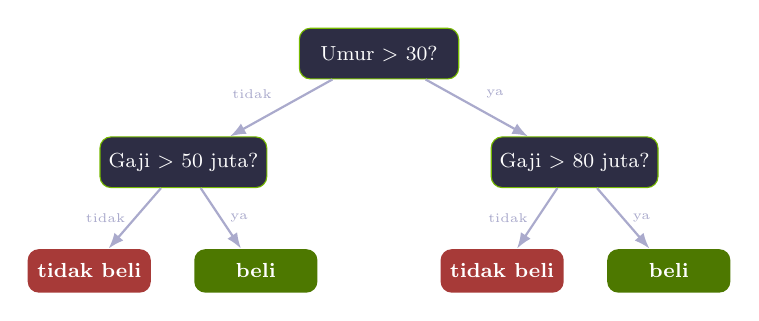
\begin{tikzpicture}[
    decision/.style={rounded corners=4pt, fill=nvcard, draw=nvgreen, text=nvwhite,
                     font=\footnotesize, minimum width=2.2cm, minimum height=0.7cm,
                     align=center},
    leafred/.style={rounded corners=4pt, fill=nvred!70!black, text=nvwhite,
                    font=\footnotesize\bfseries, minimum width=1.7cm, minimum height=0.6cm},
    leafgreen/.style={rounded corners=4pt, fill=nvgreen!65!black, text=nvwhite,
                      font=\footnotesize\bfseries, minimum width=1.7cm, minimum height=0.6cm},
    edg/.style={draw=nvgray, thick, -{Latex[length=2mm]}},
    lbl/.style={font=\tiny, text=nvgray},
    scale=0.92, every node/.style={transform shape}]
    \node[decision] (root) at (0,0) {Umur $>$ 30?};
    \node[decision] (L1) at (-2.7,-1.5) {Gaji $>$ 50 juta?};
    \node[decision] (R1) at (2.7,-1.5) {Gaji $>$ 80 juta?};
    \node[leafred]   (LL) at (-4.0,-3.0) {tidak beli};
    \node[leafgreen] (LR) at (-1.7,-3.0) {beli};
    \node[leafred]   (RL) at (1.7,-3.0) {tidak beli};
    \node[leafgreen] (RR) at (4.0,-3.0) {beli};
    \draw[edg] (root) -- node[lbl, above left] {tidak} (L1);
    \draw[edg] (root) -- node[lbl, above right] {ya} (R1);
    \draw[edg] (L1) -- node[lbl, left] {tidak} (LL);
    \draw[edg] (L1) -- node[lbl, right] {ya} (LR);
    \draw[edg] (R1) -- node[lbl, left] {tidak} (RL);
    \draw[edg] (R1) -- node[lbl, right] {ya} (RR);
  \end{tikzpicture}
  \end{center}
  \vspace{0.2em}
  {\footnotesize\color{nvgray}Satu baris data menuruni pohon lewat satu jalur saja, lalu memakai
  label di ujung jalur itu sebagai prediksi.}
\end{frame}

% ----------------------------------------------------------
% FRAME 40 — Mekanisme decision tree
% ----------------------------------------------------------
\begin{frame}{Decision tree: bagaimana pertanyaannya dipilih}
  \vspace{0.5em}
  \begin{itemize}\setlength\itemsep{0.45em}
    \item Di tiap simpul, model mencoba banyak pasangan feature dan ambang, lalu memilih
          pasangan yang paling memisahkan kelas.
    \item Ukuran pemisahannya adalah \textbf{gini}: makin kecil, makin murni isi tiap cabang.
    \item Proses itu diulang pada tiap cabang sampai simpulnya murni atau batas yang kamu
          pasang tercapai.
    \item Batasnya yang penting: \texttt{max\_depth} (kedalaman) dan
          \texttt{min\_samples\_leaf} (isi minimum tiap ujung).
  \end{itemize}
  \vspace{0.6em}
  {\footnotesize\color{nvgray}Karena tiap pertanyaan hanya membandingkan satu feature dengan satu
  angka, batas keputusannya selalu sejajar sumbu feature.}
\end{frame}

% ----------------------------------------------------------
% FRAME 41 — Kapan pakai & jebakan decision tree
% ----------------------------------------------------------
\begin{frame}{Decision tree: kapan pakai dan jebakannya}
  \vspace{0.4em}
  \kapan{
    \item aturan hasilnya perlu dibaca orang lain
    \item feature bercampur angka dan kategori
    \item scaling tidak dilakukan; pohon tidak membutuhkannya
  }{
    \item batas antar kelas miring atau melengkung halus
    \item datanya sedikit dan pohonnya dibiarkan tumbuh bebas
    \item kamu butuh prediksi yang stabil terhadap perubahan kecil data
  }
  \vspace{1.0em}
  \jebakan{tanpa batas kedalaman, pohon dapat menghafal data train sampai errornya nol dan
  hasilnya jatuh di data baru. Pilih kedalamannya dengan cross-validation.}
\end{frame}

% ----------------------------------------------------------
% FRAME 42 — Intuisi: KNN
% ----------------------------------------------------------
\begin{frame}
  \intuisi{KNN: lihat data terdekat, ambil suara terbanyak}
  \vspace{0.3em}
  \begin{columns}[T]
    \begin{column}{0.5\textwidth}
      \begin{center}
      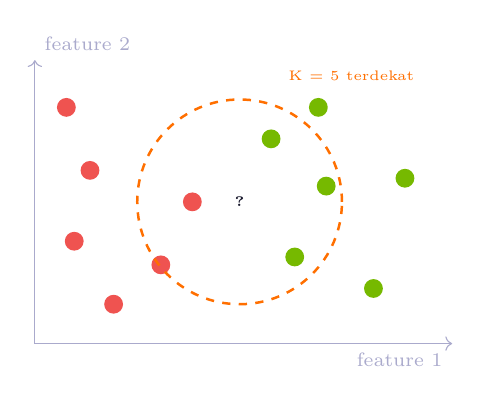
\begin{tikzpicture}[scale=1.0, font=\scriptsize]
        \draw[nvgray, ->] (-0.1,-0.1) -- (5.2,-0.1) node[below left, text=nvgray] {feature 1};
        \draw[nvgray, ->] (-0.1,-0.1) -- (-0.1,3.5) node[above right, text=nvgray] {feature 2};
        \foreach \x/\y in {0.4/1.2, 0.9/0.4, 1.5/0.9, 0.6/2.1, 1.9/1.7, 0.3/2.9}
          \fill[nvred] (\x,\y) circle (3.4pt);
        \foreach \x/\y in {3.2/1.0, 3.6/1.9, 4.2/0.6, 2.9/2.5, 3.5/2.9, 4.6/2.0}
          \fill[nvgreen] (\x,\y) circle (3.4pt);
        \fill[nvwhite] (2.5,1.7) circle (4pt);
        \node[text=nvbg, font=\tiny\bfseries] at (2.5,1.7) {?};
        \draw[nvorange, dashed, line width=0.9pt] (2.5,1.7) circle (1.3);
        \node[text=nvorange, font=\tiny, anchor=west] at (3.0,3.3) {K = 5 terdekat};
      \end{tikzpicture}
      \end{center}
    \end{column}
    \begin{column}{0.48\textwidth}
      \vspace{0.5em}
      \begin{itemize}\setlength\itemsep{0.45em}
        \item Titik putih adalah data baru yang belum punya label.
        \item Lima data train terdekat: tiga hijau, dua merah. Prediksinya hijau.
      \end{itemize}
      \vspace{0.6em}
      \nvbox{Intinya}{Tetangga di sini berarti data train yang paling dekat menurut jarak pada
      feature, bukan tetangga dalam arti sehari-hari.}
    \end{column}
  \end{columns}
\end{frame}

% ----------------------------------------------------------
% FRAME 43 — Mekanisme KNN
% ----------------------------------------------------------
\begin{frame}{KNN: jarak, K, dan suara mayoritas}
  \vspace{0.2em}
  \begin{center}
    \nvbox{Jarak Euclidean antara dua baris data}{
      \centerline{$\displaystyle d(a,b) \;=\; \sqrt{\sum_{j=1}^{m}\bigl(a_j - b_j\bigr)^2}$}
    }
  \end{center}
  \vspace{0.2em}
  \begin{itemize}\setlength\itemsep{0.3em}
    \item $a$ dan $b$ dua baris data, $m$ jumlah feature, dan $K$ jumlah tetangga yang dilihat.
    \item Hitung jarak data baru ke data train, ambil K yang terdekat, lalu pakai kelas
          terbanyak di antara mereka.
    \item K kecil membuat prediksi mengikuti tiap variasi acak di sekitarnya. K besar membuat
          batasnya terlalu rata dan pola lokal hilang.
    \item Tidak ada parameter yang dilatih. Semua pekerjaan terjadi saat prediksi.
  \end{itemize}
\end{frame}

% ----------------------------------------------------------
% FRAME 44 — Kapan pakai & jebakan KNN
% ----------------------------------------------------------
\begin{frame}{KNN: kapan layak dicoba}
  \vspace{0.7em}
  \begin{itemize}\setlength\itemsep{0.7em}
    \item Mulai dari data kecil dengan sedikit feature yang relevan.
    \item Prediksi dapat melambat saat data train membesar, karena pencarian tetangga
          dilakukan setiap kali memprediksi.
    \item Jika skala feature berbeda, lakukan scaling agar perhitungan jarak tidak didominasi
          satu feature.
  \end{itemize}
  \vspace{1.0em}
  \jebakan{gaji ditulis dalam juta rupiah dan umur dalam tahun. Tanpa scaling, selisih gaji
  yang rentang nilainya jauh lebih besar hampir menentukan seluruh jaraknya.}
\end{frame}

% ----------------------------------------------------------
% FRAME 45 — Intuisi: SVM
% ----------------------------------------------------------
\begin{frame}
  \intuisi{SVM: cari jalan paling lebar di antara dua kelas}
  \vspace{0.2em}
  \begin{columns}[T]
    \begin{column}{0.52\textwidth}
      \begin{center}
        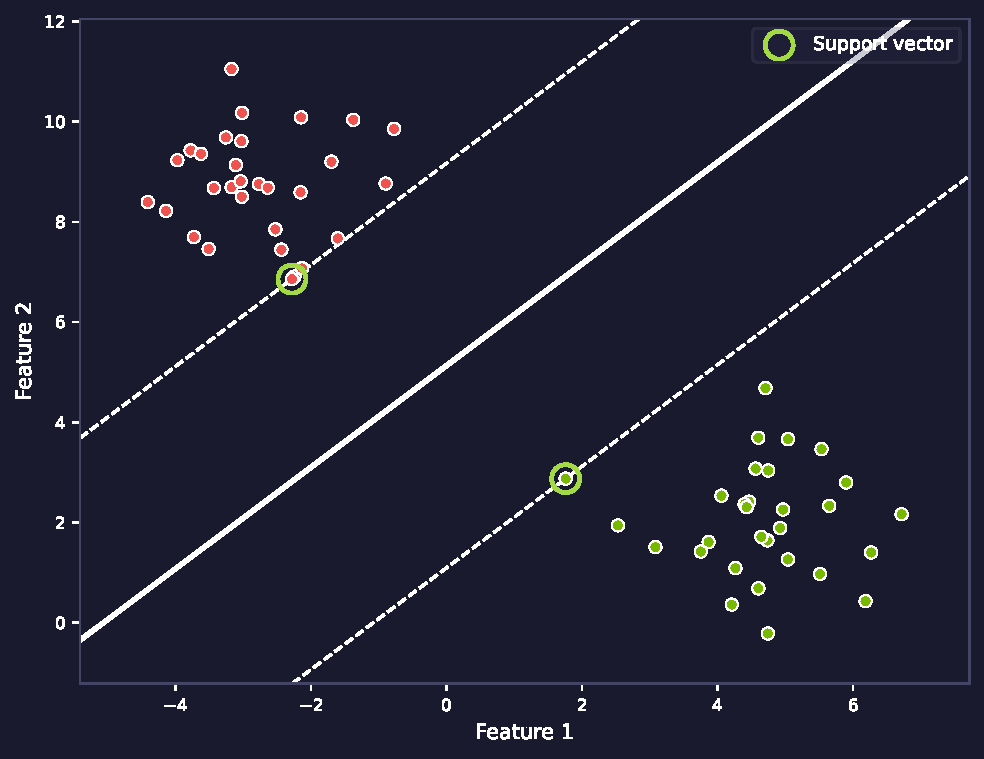
\includegraphics[width=\textwidth, height=4.6cm, keepaspectratio]{figures/svm_margin.pdf}
      \end{center}
    \end{column}
    \begin{column}{0.46\textwidth}
      \vspace{0.3em}
      \begin{itemize}\setlength\itemsep{0.45em}
        \item Di antara semua garis pemisah, SVM memilih yang jarak ke kelas terdekat di kedua
              sisinya paling lebar.
        \item Titik yang menempel di tepi jalan itu disebut support vector.
      \end{itemize}
      \vspace{0.6em}
      \nvbox{Intinya}{Hanya titik di dekat batas yang menentukan posisi garisnya. Titik yang
      jauh boleh digeser tanpa mengubah hasilnya.}
    \end{column}
  \end{columns}
\end{frame}

% ----------------------------------------------------------
% FRAME 46 — Mekanisme SVM
% ----------------------------------------------------------
\begin{frame}{SVM: margin, C, dan kernel}
  \vspace{0.5em}
  \begin{itemize}\setlength\itemsep{0.45em}
    \item \textbf{Margin} adalah lebar jalan antara batas keputusan dan support vector
          terdekat. Pelatihan memaksimalkan lebar itu.
    \item \textbf{C} mengatur seberapa banyak titik boleh masuk ke dalam margin. C kecil
          memberi margin lebar dengan beberapa pelanggaran; C besar memaksa margin sempit yang
          rapat mengikuti data train.
    \item \textbf{Kernel RBF} mengangkat data ke ruang berdimensi lebih tinggi, tempat kedua
          kelas dapat dipisahkan bidang datar. Kembali ke dua feature semula, batasnya terlihat
          melengkung.
    \item \texttt{gamma} pada RBF mengatur seberapa lokal pengaruh satu titik.
  \end{itemize}
\end{frame}

% ----------------------------------------------------------
% FRAME 47 — Kapan pakai & jebakan SVM
% ----------------------------------------------------------
\begin{frame}{SVM: kapan pakai dan jebakannya}
  \vspace{0.4em}
  \kapan{
    \item jumlah feature banyak dibanding jumlah baris
    \item batas antar kelas cukup tegas
    \item kamu bersedia mencari pasangan C dan \texttt{gamma} lewat cross-validation
  }{
    \item data trainnya ratusan ribu baris
    \item probabilitas kelas dibutuhkan langsung dari model
    \item hasilnya harus dijelaskan sebagai aturan per feature
  }
  \vspace{1.0em}
  \jebakan{kernel RBF melambat cepat saat data membesar, dan SVM mengukur jarak. Jika skala
  feature berbeda, lakukan scaling lebih dulu.}
\end{frame}

% ----------------------------------------------------------
% FRAME 48 — Empat model, satu dataset
% ----------------------------------------------------------
\begin{frame}{Empat model, satu dataset}
  \vspace{0.2em}
  \begin{center}
    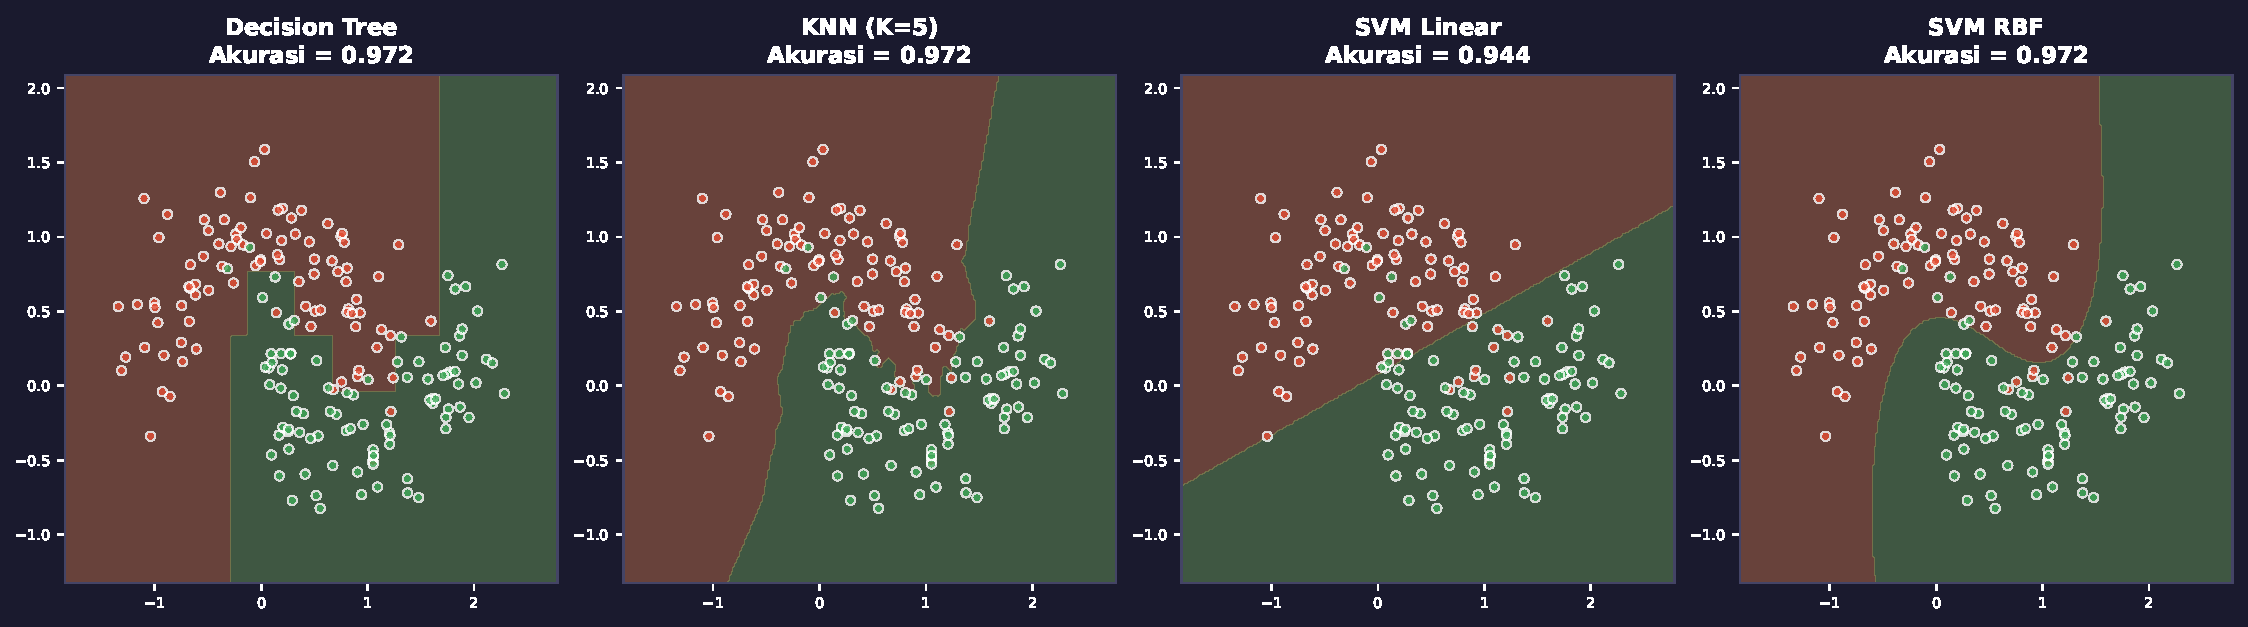
\includegraphics[width=\textwidth, height=4.1cm, keepaspectratio]{figures/decision_boundaries.pdf}
  \end{center}
  \vspace{0.3em}
  \begin{itemize}\setlength\itemsep{0.3em}
    \item Data yang sama, empat batas keputusan yang berbeda: bentuk batasnya mengikuti cara
          model itu menarik keputusan.
    \item Karena itu perbandingan model selalu dilakukan pada satu split dan satu metrik yang
          sama.
  \end{itemize}
\end{frame}

% ----------------------------------------------------------
% FRAME 49 — Ringkasan Act 4
% ----------------------------------------------------------
\begin{frame}{Ringkasan Act 4: kapan pakai model yang mana}
  \vspace{0.4em}
  \begin{center}
  {\small\renewcommand{\arraystretch}{1.25}
  \begin{tabular}{@{}llccl@{}}
    \toprule
    \rowcolor{nvcard}\color{nvgreen}\textbf{Model} &
    \color{nvgreen}\textbf{Bentuk batas keputusan} &
    \color{nvgreen}\textbf{Scaling} &
    \color{nvgreen}\textbf{Prediksi} &
    \color{nvgreen}\textbf{Dibaca orang} \\
    \midrule
    Logistic regression & garis lurus & perlu & cepat & mudah \\
    \rowcolor{nvcard!60!nvbg} Decision tree & sejajar sumbu feature & tidak perlu & cepat & mudah \\
    KNN & mengikuti sebaran data & perlu & melambat & sulit \\
    \rowcolor{nvcard!60!nvbg} SVM linear & garis lurus & perlu & sedang & sedang \\
    SVM RBF & melengkung & perlu & lambat & sulit \\
    \bottomrule
  \end{tabular}}
  \end{center}
  \vspace{0.7em}
  {\footnotesize\color{nvgray}Kolom scaling berlaku kalau skala feature berbeda-beda. Tabel ini
  membantu memilih kandidat awal; keputusannya tetap dari hasil di data validation.}
\end{frame}

\end{document}
